\section{Exercises}

%%%%%%%%%%%%%%%%%%%%%%%%%%%%%%%%%%%%%

\subsection{Case study}

%%%%%%%%%%%%%%%%%%%%%%%%%%%%%%%%%%%%%

\Comment{TO DO: Check on linking to articles, will be implemented (if possible) after Chris' review.}

% 1

\eoce{\qt{Migraine and accupuncture}
A migraine is a common type of headache, which patients sometimes wish to treat with acupuncture. To determine whether acupuncture relieves migraine pain, researchers conducted a randomized controlled study where 89 females diagnosed with migraine headaches were randomly assigned to treatment and control groups. 43 patients in the treatment group received acupuncture specifically designed to treat migraines. 46 patients in the control group received placebo acupuncture (needle insertion at nonacupoint locations). 24 hours after patients received acupuncture they were asked if they were pain free. The results are summarized in the contingency table below. \footfullcite{Allais:2011}

\begin{minipage}[c]{0.35\textwidth}
\centering
\begin{tabular}{ll  cc c} 
			&				& \multicolumn{2}{c}{\textit{Pain free}} \\
\cline{3-4}
			&							& Yes 	& No 	& Total	\\
\cline{2-5}
							&Treatment 	& 10	 	& 33		& 43 	\\
\raisebox{1.5ex}[0pt]{\emph{Group}}	& Control		& 2	 	& 44 	 	& 46 \\
\cline{2-5}
							&Total		& 12		& 77		& 89
\end{tabular}
\end{minipage}
\begin{minipage}[c]{0.05\textwidth}
$\:$
\end{minipage}
\begin{minipage}[c]{0.2\textwidth}
\begin{center}
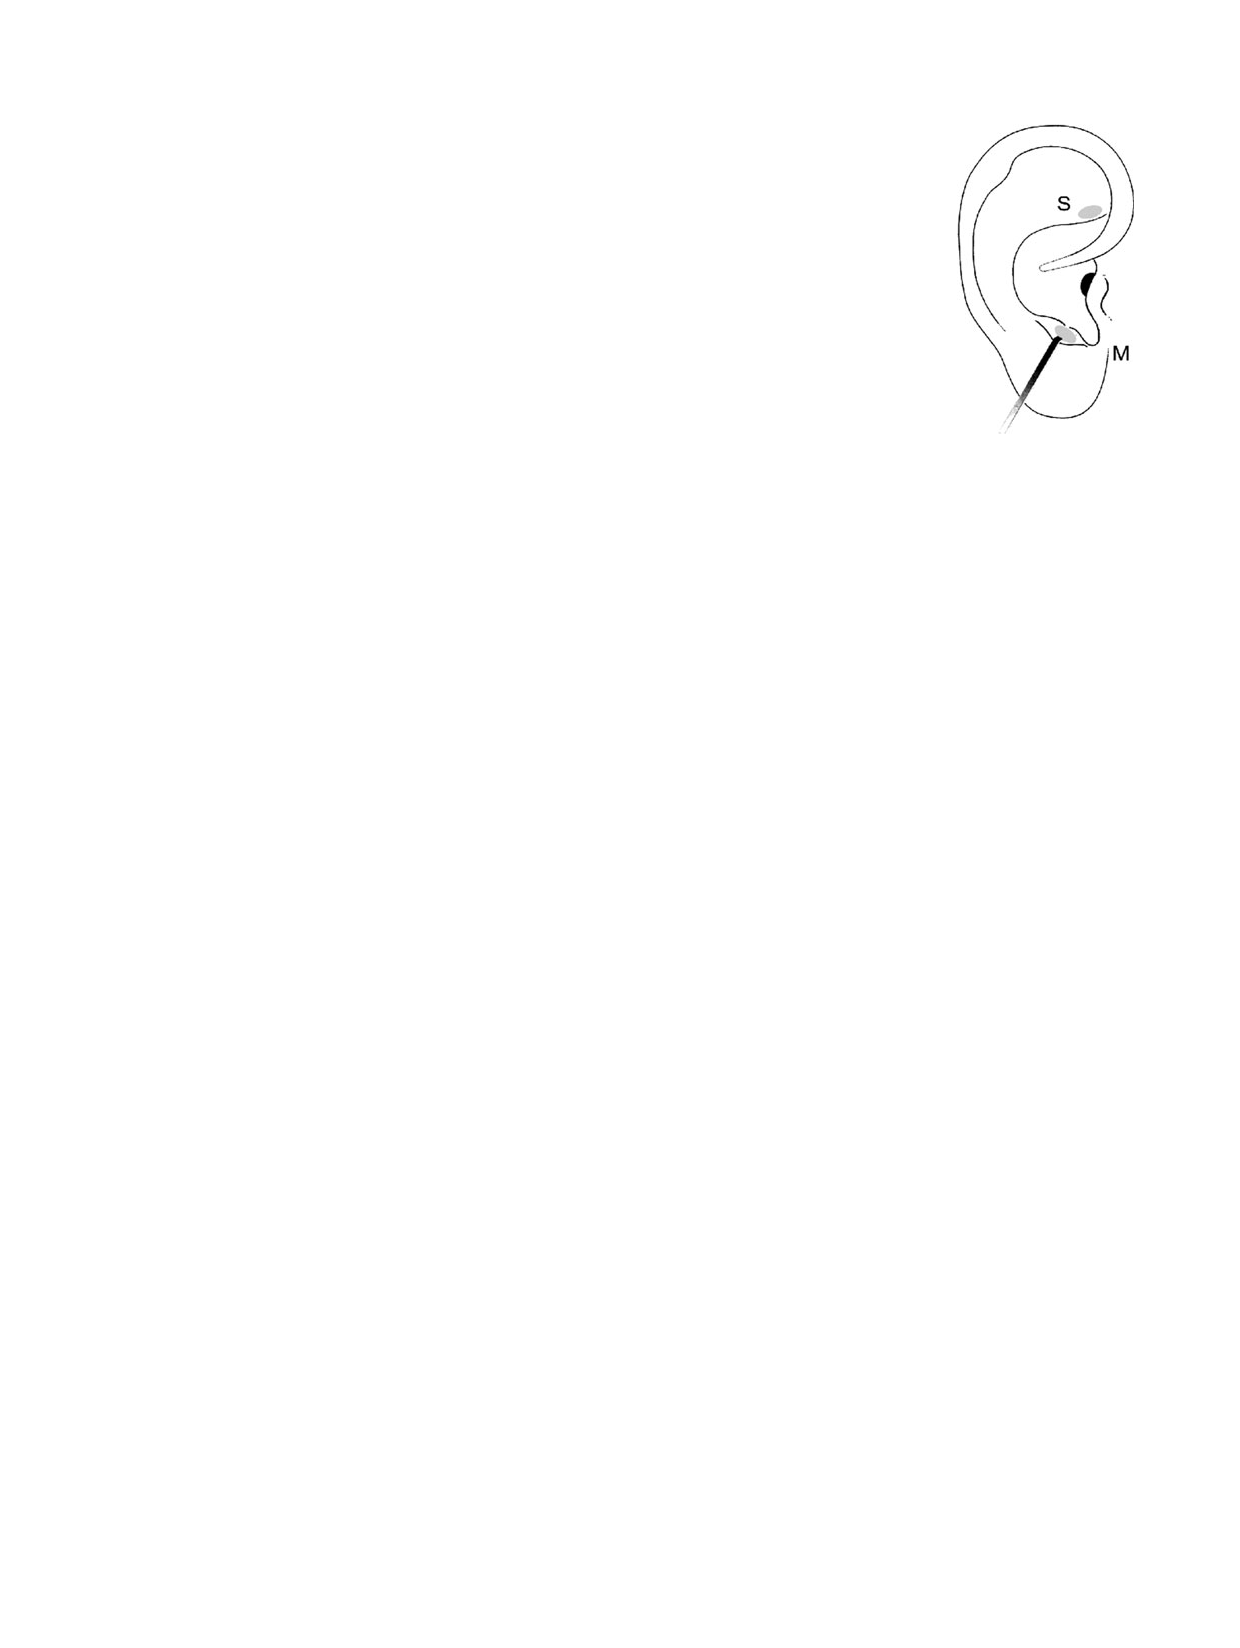
\includegraphics[width = \textwidth]{01/figures/eoce/images/earacupuncture}
\end{center}
\end{minipage}
\begin{minipage}[c]{0.3\textwidth}
{\footnotesize Figure from the original paper displaying the appropriate area (M) versus the inappropriate area (S) used in the treatment of migraine attacks.}
\end{minipage}
\begin{parts}
\item What percent of patients in the treatment group were pain free 24 hours after receiving acupuncture? What percent in the control group?
\item At first glance, does acupuncture appear to be an effective treatment for migraines? Explain your reasoning.
\item Do the data provide convincing evidence that there is a real pain reduction for those patients in the treatment group? Or do you think that the observed difference might just be due to chance?
\end{parts}
}
{
\begin{parts}
\item Percent pain free in the treatment group: $10/43 = 0.23 \rightarrow 23\%$. \\
Percent pain free in the control group: $2/46 = 0.04 \rightarrow 4\%$.
\item While 23\% of the patients in the treatment group were pain free 24 hours after receiving acupuncture, only 4\% of patients who received the placebo (control) did. There is a 19\% difference between the pain reduction rates in the two groups. At first glance, it appears patients in the treatment group are more likely to experience pain reduction from the acupuncture treatment.
\item Answers may vary. Here are two possible answers. (1) We could get slightly different group estimates even if there is no real difference. Though the difference is big, I'm skeptical the results show a real difference and think this might be due to chance. (2) The difference in these rates looks pretty big, and so I suspect acupuncture is having a positive impact on pain.
\end{parts}
}

% 2

\eoce{\qt{Sinusitis and antibiotics} Researchers studying the effect of antibiotic treatment for acute sinusitis over symptomatic treatments randomly assigned 166 adults diagnosed with acute sinusitis to treatment and control groups. Study participants received a 10-day course of amoxicillin (an antibiotic)  or placebo similar in appearance and taste and dispensed in the same fashion. The placebo consisted of symptomatic treatments such as acetaminophen, nasal decongestants, etc. At the end of the 10-day period patients were asked if they experienced significant improvement in symptoms since the beginning of the study. The distribution of responses are summarized below. \footfullcite{Garbutt:2012}
\begin{center}
\begin{tabular}{ll  cc c} 
			&				& \multicolumn{2}{c}{\textit{Self-reported significant}} \\
			&				& \multicolumn{2}{c}{\textit{improvement in symptoms}} \\
\cline{3-4}
			&							& Yes 	& No 	& Total	\\
\cline{2-5}
							&Treatment 	& 66	 	& 19		& 85 	\\
\raisebox{1.5ex}[0pt]{\emph{Group}}	& Control		& 65	 	& 16 	 	& 81 \\
\cline{2-5}
							&Total		& 131	& 35		& 166
\end{tabular}
\end{center}
\begin{parts}
\item What percent of patients in the treatment group experienced significant improvement in symptoms? What percent in the control group?
\item At first glance, which treatment appears to be more effective for sinusitis?
\item Do the data provide convincing evidence that there is a difference in the improvement rates of sinusitis symptoms? Or do you think that the observed difference might just be due to chance?
\end{parts}
}
{
\begin{parts}
\item Percent of patients in the treatment group with self-reported significant improvement in symptoms: $66/85 = 0.78 \rightarrow 78\%$. \\
Percent of patients in the control group with self-reported significant improvement in symptoms: $65/81 = 0.80 \rightarrow 80\%$.
\item 78\% of patients in the treatment and 80\% of patients in the control group reported significant improvement in symptoms; therefore at a first glance the non-antibiotic treatment appears to be more effective for the treatment of sinusitis.
\item Even if the two treatments had the same effect on the improvement rates of sinusitis symptoms, typical we would not get the exact same rates in symptom improvement in each group. The difference of 2\%, which separates the groups by just one or two successful treatments, seems like it could be due to just chance. (The best answers will include a component regarding uncertainty.)
\end{parts}
}

%%%%%%%%%%%%%%%%%%%%%%%%%%%%%%%%%%%%%

\subsection{Data basics}

%%%%%%%%%%%%%%%%%%%%%%%%%%%%%%%%%%%%%

% 3

\eoce{\qt{Identify study components, Part I} Identify (i) the cases, (ii) the variables and their types, and (iii) the main research question in the studies described below.
\begin{parts}
\item Researchers collected data to examine the relationship between pollutants and preterm births in Southern California. During the study air pollution levels were measured by air quality monitoring stations. Specifically, levels of of carbon monoxide were recorded in parts per million, nitrogen dioxide and ozone in parts per hundred million, and coarse particulate matter (PM$_{10}$) in $\mu g/m^3$. Length of gestation data were collected on 143,196 births between the years 1989 and 1993 and air pollution exposure during gestation was calculated for each birth. The analysis suggested that increased ambient PM$_{10}$ and, to a lesser degree, CO concentrations may contribute to the occurrence of preterm births. \footfullcite{Ritz+Yu+Chapa+Fruin:2000}
\item The Buteyko method is a shallow breathing technique developed by Konstantin Buteyko, a Russian doctor, in 1952. Anecdotal evidence suggests that the Buteyko method can reduce asthma symptoms and improve quality of life. In a study aimed to determine the effectiveness of this method, researchers recruited 600 asthma patients aged 18-69 who relied on medication for asthma treatment. These patients were split into two research groups: one practiced the Buteyko method and the other did not. Patients were scored on quality of life, activity, asthma symptoms, and medication reduction on a scale from 0 to 10. On average, the participants in the Buteyko group experienced a significant reduction in asthma symptoms, and an improvement in quality of life. \footfullcite{McDowan:2003}
\end{parts}
}
{
\begin{parts}
\item 
\begin{subparts}
\item The cases are 143,196 eligible study subjects who were born in Southern California between 1989 and 1993.
\item The variables are measurements of carbon monoxide (CO), nitrogen dioxide, ozone, and particulate matter less than 10$\mu$m (PM$_{10}$) collected at air-quality-monitoring stations as well as length of gestation. All of these variables are continuous numerical variables.
\item The research question was ``Is there an association between air pollution exposure and preterm births?" 
\end{subparts}

\item 
\begin{subparts}
\item The cases are 600 adult patients aged 18-69 years diagnosed and currently treated for asthma. 
\item The variables were whether or not the patient practiced the Buteyko method (categorical) and measures of quality of life, activity, asthma symptoms and medication reduction of the patients (categorical, ordinal). It may also be reasonable to treat the ratings on a scale of 1 to 10 as discrete numerical variables.
\item The research question was ``Do asthmatic patients who practice the Buteyko method experience improvement in their condition?"
\end{subparts}

\end{parts}
}\label{components1}

% 4

\eoce{\qt{Identify study components, Part II} Identify (i) the cases, (ii) the variables and their types, and (iii) the main research question of the studies described below.
\begin{parts}
\item While obesity is measured based on body fat percentage (more than 35\% body fat for women and more than 25\% for men), measuring body fat percentage accurately is difficult. Therefore body mass index (BMI), ratio $\frac{weight}{height^2}$, is often used as an alternative indicator for obesity. A common criticism of BMI is that it assumes the same relative body fat percentage regardless of age, sex, or ethnicity. In order to determine how useful BMI is for predicting body fat percentage across age, sex and ethnic groups, researchers studied 202 black and 504 white adults who volunteered to be a part of this study, who resided in or near New York City, were ages 20-94 years old, and had BMIs of 18-35 kg/m$^2$. Participants reported their age, sex and ethnicity and were measured for weight, height. Body fat percentage was measured by submerging the participants in water. \footfullcite{Gallagher:1996} \label{BMIAgeSexEth}

\item In a study of the relationship between socio-economic class and unethical behavior, 129 University of California at Berkeley undergraduates were asked to identify themselves as having low or high social-class by comparing themselves to others with the most (least) money, most (least) education, and most (least) respected jobs. They were also presented  with a jar of individually wrapped candies and informed that they were for children in a nearby laboratory, but that they could take some if they wanted. Participants completed unrelated tasks and them reported the number of candies they had taken. It was found that those in the upper-class rank condition took more candy than did those in the lower-rank condition. \footfullcite{Piff:2012}
\end{parts}
}
{
\begin{parts}
\item 
\begin{subparts}
\item The cases are 202 black and 504 white adults who resided in or near New York City, were ages 20-94 years, and had BMIs of 18-35 kg/m$^2$.
\item The variables are age (numerical, discrete or continuous, depending on whether or not it's recorded in years), sex (categorical), ethnicity (categorical), weight, height, body fat percentage (numerical, continuous).
\item The research question was ``How useful is BMI for predicting body fat percentage across age, sex and ethnic groups?"
\end{subparts}
\item 
\begin{subparts}
\item The cases are 129 University of California at Berkeley undergraduates.
\item The variables are social-class rank (categorical) and number of candies taken (numerical, discrete).
\item The research question was ``Is there a difference between the unethical behaviors of people who identify themselves as having low and high social-class rank?"
\end{subparts}

\end{parts}
}\label{components2}

% 5

\eoce{\qt{Fisher's irises} Sir Ronald Aylmer Fisher was an English statistician, evolutionary biologist and geneticist who worked on a data set that contained sepal length and width, and petal length and width from three species of iris flowers (\textit{setosa}, \textit{versicolor} and \textit{virginica}). There were 50 flowers from each species in the data set. \footfullcite{Fisher:1936,irisPic}
\begin{center}
\begin{minipage}[c]{0.55\textwidth}
\begin{parts}
\item How many cases were included in the data?
\item How many numerical variables are included in the data? Indicate what they are, and if they are continuous or discrete.
\item How many categorical variables are included in the data, and what are they? List the corresponding levels (categories).
\end{parts}
\end{minipage}
\begin{minipage}[c]{0.4\textwidth}
\begin{center}
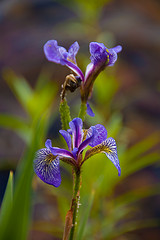
\includegraphics[width = 30mm]{01/figures/eoce/images/irisversicolor}
\end{center}
\end{minipage}
\end{center}
}
{
\begin{parts}
\item There are 50 * 3 = 150 cases included in this data set.
\item There are 4 numerical variables in the data: sepal length, sepal width, petal length and petal width, and they are all continuous numerical variables.
\item There is only one categorical variable in the data, which is species. It has 3 levels: setosa, versicolor, and virginica.
\end{parts}
}

% 6

\eoce{\qt{Smoking habits of UK residents} A survey was conducted to study the smoking habits of UK residents. Below is a data matrix displaying a portion of the data collected in this survey. Note that ``$\pounds$" stands for British Pounds Sterling and ``cig" stands for cigarettes. \footfullcite{data:smoking}
\begin{table}[h]
\begin{center}
\scriptsize{
\begin{tabular}{rccccccc}
  \hline
 & gender & age & marital & grossIncome & smoke & amtWeekends & amtWeekdays \\ 
  \hline
1 & Female &  42 & Single & Under $\pounds$2,600 & Yes &  12 cig/day &  12 cig/day \\ 
2 & Male &  44 & Single & $\pounds$10,400 to $\pounds$15,600 & No & N/A & N/A \\ 
3 & Male &  53 & Married & Above $\pounds$36,400 & Yes &   6 cig/day &   6 cig/day \\ 
\vdots & \vdots &  \vdots & \vdots & \vdots & \vdots & \vdots & \vdots \\ 
1691 & Male &  40 & Single & $\pounds$2,600 to $\pounds$5,200 & Yes &   8 cig/day &   8 cig/day \\   
   \hline
\end{tabular}
}
\end{center}
\end{table}
\begin{parts}
\item What does each row of the data matrix represent?
\item How many participants were included in the survey?
\item Indicate if the variables in the study are numerical or categorical. If numerical, identify as continuous or discrete. If categorical, indicate if the variable is ordinal.
\end{parts}
}
{
\begin{parts}
\item Each row of the data matrix represents a participant in the survey.
\item There are 1,691 participants in the survey.
\item The table below lists the types of the variables included in the study.
\begin{center}
\begin{tabular}{l l}
  \hline
\textbf{variable} & \textbf{type} \\ 
\hline
gender & categorical \\ 	
age & numerical, continuous (recorded as rounded to whole years) \\
maritalStatus & categorical \\
grossIncome & ordinal* \\
smoke & categorical \\
amtWeekends & numerical, discrete \\ 
amtWeekdays & numerical, discrete \\
  \hline
\end{tabular}
\end{center}
*Note that income is a continuous numerical variable, but in this survey it is recorded as an ordinal variable.
\end{parts}
}\label{UKSmoking_datamatrix}

%%%%%%%%%%%%%%%%%%%%%%%%%%%%%%%%%%%%%

\subsection{Overview of data collection principles}

%%%%%%%%%%%%%%%%%%%%%%%%%%%%%%%%%%%%%

% 7

\eoce{\qt{Generalizability and causality, Part I} Identify the population of interest and the sample in the the studies described in Exercise~\ref{components1}. Also comment on whether or not the results of the study can be generalized to the population, and if the findings of the study can be used to establish causal relationships.
}
{
\begin{parts}
\item The population of interest is all births. The sample consists of the 143,196 births between 1989 and 1993 in Southern California. If births in this time span at the geography can be considered to be representative of all births, then the results are generalizable to the population of Southern California. However, since the study is observational the findings cannot be used to establish causal relationships.
\item The population is all 18-69 year olds diagnosed and currently treated for asthma. The sample is the 600 adult patients aged 18-69 years diagnosed and currently treated for asthma. Since the sample is not random (voluntary) the results cannot be generalized to the population at large. However, since the study is an experiment, the findings can be used to establish causal relationships.
\end{parts}
}

% 8

\eoce{\qt{Generalizability and causality, Part II} Identify the population and the sample in the the studies described in Exercise~\ref{components2}. Also comment on whether or not the results of the study can be generalized to the population, and if the findings of the study can be used to establish causal relationships.
}
{
\begin{parts}
\item The population of interest is all adults. The sample is the 202 black and 504 white men and women who resided in or near New York City and had BMIs of 18-35 kg/m$^2$.  The sample is voluntary so the results cannot be generalized to the population at large. Since it doesn't appear to be representative of the population at large since the racial diversity of the subjects is limited. In addition, since the study is observational the findings cannot be used to establish causal relationships. 
\item The population is not defined but it's likely intended to be all people. The sample is 129 UC Berkeley undergraduates. We are not told how the sample is collected, however, it is certainly not representative of the population at large since it consists only of undergraduate students at UC Berkeley. However, this is an experiment therefore the findings of the study can be used to establish causal relationships.
\end{parts}
}

% 9

\eoce{\qt{GPA and study time} A survey was conducted on 218 undergraduates from Duke University who took an introductory statistics course in Spring 2012 semester. Among many other questions, this survey asked them about their GPA and the number of hours they spend studying per week. The scatterplot below displays the relationship between these two variables.

\noindent\begin{minipage}[c]{0.5\textwidth}
\begin{parts}
\item What is the explanatory variable and what is the response variable?
\item Describe the relationship between the two variables. Make sure to discuss unusual observations, if any.
\item Is this an experiment or an observational study?
\item Can we conclude that studying longer hours leads to higher GPAs?
\end{parts}
\end{minipage}
\begin{minipage}[c]{0.5\textwidth}
\begin{center}
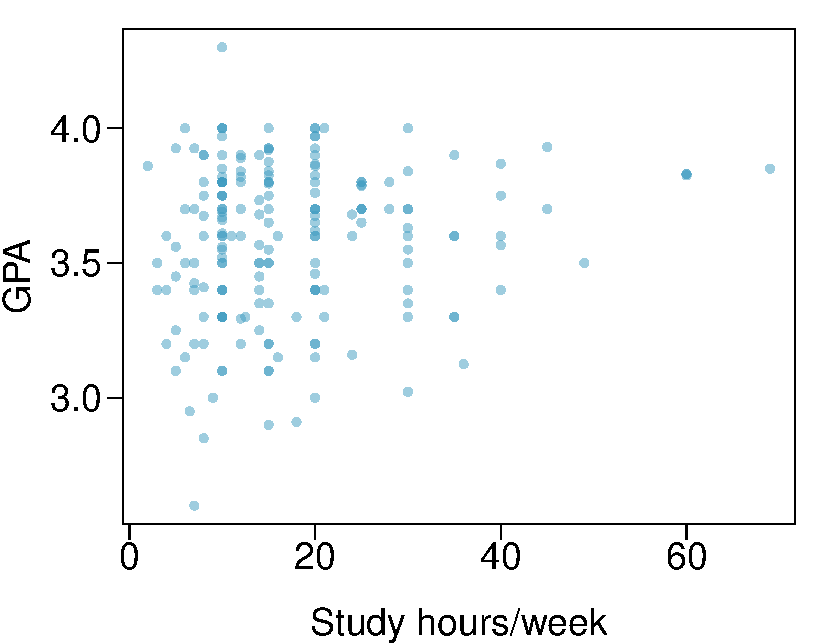
\includegraphics[width = 0.825\textwidth]{01/figures/eoce/gpaStudy/gpaStudy}
\end{center}
\end{minipage}
}
{
\begin{parts}
\item The explanatory variable is the number of study hours per week, and the response variable is GPA.
\item There is a somewhat weak positive relationship between the two variables, though the data become more sparse as the number of study hours increases. One responded reported a GPA above 4.0, which is clearly a data error. Also, there are a few respondents who reported unusually high study hours (60 and 70 hours/week). It should also be noted that the variability in GPA is much higher for students who study less than those who study more, also might be due to the fact that there aren't many respondents who reported studying higher hours.
\item This is an observational study.
\item Since this is an observational study, we cannot conclude that there is a causal relationship between the two variables even though there appears to be an association.
\end{parts}
}

% 10

\eoce{\qt{Income and education} The scatterplot below shows the relationship between per capita income (in thousands) and percent of population with a bachelor's degree in 3,143 counties in the US in 2010.

\noindent\begin{minipage}[c]{0.5\textwidth}
\begin{parts}
\item What are the explanatory and response variables?
\item Describe the relationship between the two variables. Make sure to discuss unusual observations, if any.
\item Can we conclude that having a bachelor's degree increases one's income?
\end{parts}
\end{minipage}
\begin{minipage}[c]{0.5\textwidth}
\begin{center}
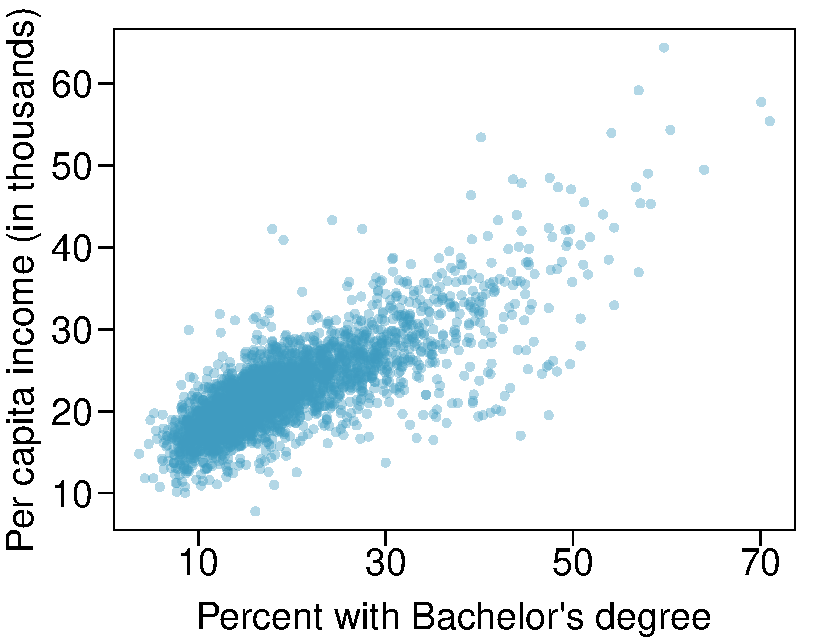
\includegraphics[width = 0.825\textwidth]{01/figures/eoce/county/county_incomeBach}
\end{center}
\end{minipage}
}
{
\begin{parts}
\item The explanatory variable is percent of population with a bachelor's degree and the response variable is per capita income (in thousands).
\item There is a strong positive linear relationship between the two variables. As the percentage of population with a bachelor's degree increases the per capita income increases as well. There are very few counties where more than 60\% of the population have a bachelor's degree and very few countries that have a more than \$50,000 in per capita income.
\item This is an observational study so we cannot make a causal statement based on the results. However, we can say that having a higher percentage of population with bachelor's degree is associated with a higher per capita income.
\end{parts}
}

%%%%%%%%%%%%%%%%%%%%%%%%%%%%%%%%%%%%%

\subsection{Observational studies and sampling strategies}

%%%%%%%%%%%%%%%%%%%%%%%%%%%%%%%%%%%%%

% 11

\eoce{\qt{Propose a sampling strategy} A large college class has 160 students. All 160 students attend the lectures together but are split into 4 groups of 40 for lab sections run by different teaching assistants. The professor wants to conduct a survey about how satisfied the students are with the course and she believes that the lab section a student is in might affect their overall satisfaction with the course.
\begin{parts}
\item What type of study is this?
\item Suggest a sampling strategy for carrying out this study and identity the type of sampling method you suggest.
\end{parts}
}
{
\begin{parts}
\item This is an observational study.
\item The professor suspects students in a given section may have similar feelings about a course. To ensure each section is reasonably represented, she may choose to randomly select a fixed number of students, say 10, from each section for a total sample size of 40 students. Since a random sample of fixed size was taken within each section in this scenario, this represents a stratified sampling.
\end{parts}
}

% 12

\eoce{\qt{Internet use and life expectancy} The scatterplot below shows the relationship between estimated life expectancy at birth as of 2012\footfullcite{data:ciaFactBookLifeExp:2012} and percentage of internet users in 2010\footfullcite{data:ITU:2012} in 208 countries.

\noindent\begin{minipage}[c]{0.5\textwidth}
\begin{parts}
\item Describe the relationship between life expectancy and percentage of internet users.
\item What type of study is this?
\item State a possible lurking variable that might explain this relationship and describe its potential effect.
\end{parts}
\end{minipage}
\begin{minipage}[c]{0.5\textwidth}
\begin{center}
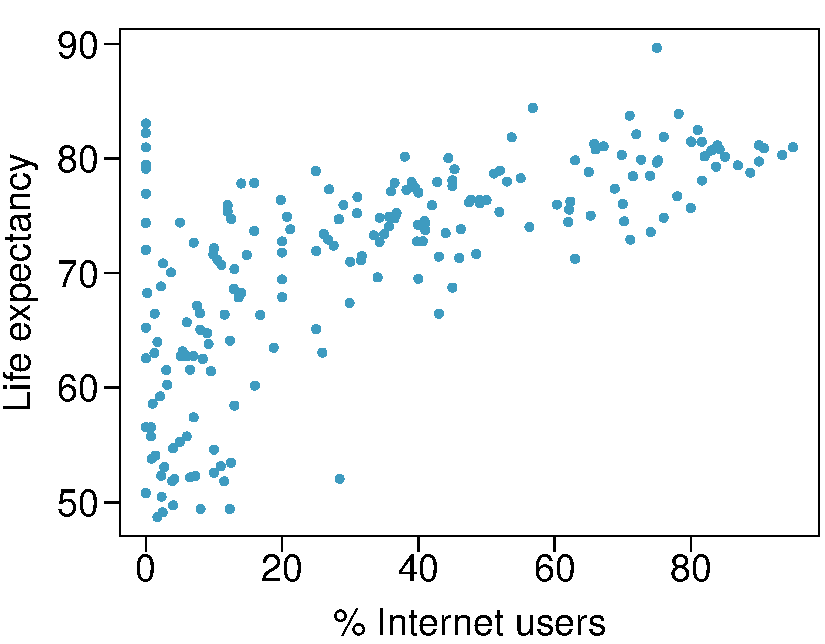
\includegraphics[width = 0.825\textwidth]{01/figures/eoce/country/county_lifeExpInter}
\end{center}
\end{minipage}
}
{
\begin{parts}
\item The two variables are positively associated. Countries in which a higher percentage of the population have access to the Internet also tend to have higher average life expectancies.
\item This is an observational study.
\item Wealth is one lurking variable. Countries with individuals who can widely afford internet can probably also afford basic medical care. (Note: Answers may vary.)
\end{parts}
}

% 13

\eoce{\qt{Random digit dialing} The Gallup Poll uses a procedure called random digit dialing (RDD) which creates phone numbers based on a list of all area codes in America, along with estimates of the number of residential households those exchanges have attached to them. This procedure is a lot more complicated than obtaining a list of all phone numbers from the phone book. Give a possible reason the Gallup Poll chooses to use RDD instead of picking phone numbers from the phone book?}
{Sampling from the phone book would introduce bias since it would miss unlisted phone numbers. If the unlisted phone numbers are missing at random this may not be a problem, but if people who choose to not list their numbers share a certain characteristic, our sample would not be able to capture such people and therefore would not be representative of the population.}

% 14

\eoce{\qt{Sampling strategies} A statistics student curious about the relationship between the amount of time students spend on social networking sites and their performance at school decides to conduct a survey. Two research strategies for collecting data are described below. Name the sampling method proposed and any bias you might expect.
\begin{parts}
\item He randomly samples 40 students from the study's population, gives them the survey, asks them to fill it out and bring it back the next day.
\item He gives out the survey only to his friends, and makes sure each one of them fills out the survey.
\item He posts a link to an online survey on his Facebook wall and asks his friends to fill out the survey.
\APVersion{\item He stands outside the student center and asks every third person that walks out the door to fill out the survey.}
\end{parts}
}
{
\begin{parts}
\item Simple random sample. Non-response bias, if only those people who have strong opinions about the survey responds his sample may not be representative of the population.
\item Convenience sample. Under coverage bias, his sample may not be representative of the population since it consists only of his friends. It is also possible that the study will have non-response bias if some choose to not bring back the survey.
\item Convenience sample. This will have a similar issues to handing out surveys to friends.
\APVersion{\item Systematic sample. There might be non-response bias, similar to when using a simple random sample. Also, there might be a sapling bias since not all students may visit the student center.}
\end{parts}
}

% 15

\eoce{\qt{Family size} Suppose we want to estimate family size, where family is defined as married or cohabiting couples and their children, if any. If we select students at random at an elementary school and ask them what their family size is, will our average be biased? If so, will it overestimate or underestimate the true value?
}
{
Yes, the estimate will be biased, and it will tend to overestimate the true family size. Notice that families without children cannot be sampled using the sampling strategy. Additionally, if a family has two children, it is twice as likely to be sampled than a family with one child since there are twice as many children included in the sample (on the average).
}

% 16

\eoce{\qt{Flawed reasoning} Identify the flaw in reasoning in the following scenarios. Explain what the individuals in the study should have done differently if they wanted to make such strong conclusions.
\begin{parts}
\item Students at an elementary school are given a questionnaire that they are required to return after their parents have completed it. One of the questions asked is, ``Do you find that your work schedule makes it difficult for you to spend time with your kids after school?" Of the parents who replied, 85\% said "no". Based on these results, the school officials conclude that a great majority of the parents have no difficulty spending time with their kids after school.
\item A survey is conducted on a simple random sample of 1,000 women who recently gave birth, asking them about whether or not they smoked during pregnancy. A follow-up survey asking if the children have respiratory problems is conducted 3 years later, however only 567 of these women are reached at the same address. The researcher reports that these 567 women represent a simple random sample of all mothers.
\item A orthopedist administers a questionnaire to 30 of his patients who do not have any joint problems and finds that 20 of them regularly go running. He concludes that running decreases the risk of joint problems.
\end{parts}
}
{
\begin{parts}
\item Non-responders may have a different response to this question. The parents who returned the surveys are probably those who do not have difficulty spending time with their kids after school. Parents who work might not have returned the surveys since they probably have a busier schedule.
\item It is unlikely that the women who were reached at the same address 3 years later are a random sample. These missing responders are probably renters (as opposed to homeowners) which means that they might be in a lower socio-economic status than the respondents.
\item First, there is no control group in this study. It may be that if we looked at 30 patients with joint problems, 20 of them regularly go running as well. Second, this is an observational study. Third, there may be lurking variables. For example, these people may go running because they are generally healthier and/or do other exercises. 
\end{parts}
}

% 17

\eoce{\qt{Reading the paper} Below are excerpts from two articles published in the \emph{New York Times}:
\begin{parts}
\item An article called \emph{Risks: Smokers Found More Prone to Dementia} states the following: \footfullcite{news:smokingDementia}
\begin{adjustwidth}{2em}{2em}
{\footnotesize ``Researchers analyzed the data of 23,123 health plan members who participated in a voluntary exam and health behavior survey from 1978 to 1985, when they were 50 to 60 years old. Twenty-three years later, about one-quarter of the group, or 5,367, had dementia, including 1,136 with Alzheimer�s disease and 416 with vascular dementia. After adjusting for other factors, the researchers concluded that pack-a-day smokers were 37 percent more likely than nonsmokers to develop dementia, and the risks went up sharply with increased smoking; 44 percent for one to two packs a day; and twice the risk for more than two packs."}
\end{adjustwidth}
Based on this study can we conclude that smoking causes dementia later in life? Explain your reasoning.
\item Another article called \emph{The School Bully Is Sleepy} states the following: \footfullcite{news:bullySleep}
\begin{adjustwidth}{2em}{2em}
{\footnotesize ``The University of Michigan study, collected survey data from parents on each child's sleep habits and asked both parents and teachers to assess behavioral concerns. About a third of the students studied were identified by parents or teachers as having problems with disruptive behavior or bullying. The researchers found that children who had behavioral issues and those who were identified as bullies were twice as likely to have shown symptoms of sleep disorders."}
\end{adjustwidth}
A friend of yours who read the article says ``The study shows that sleep disorders lead to bullying in school children." Is this statement justified? If not, how best can you describe the conclusion that can be drawn from this study?
\end{parts}
}
{
\begin{parts}
\item No, this was an observational study, and we cannot make such a causal statement based on an observational study.
\item This statement is not justified because it implies a causal association between sleep disorders and bullying, which we can't conclude based on this observational study. Instead, a better conclusion would be ``School children identified as bullies are more likely to suffer from sleep disorders than non-bullies."
\end{parts}
}

% 18

\eoce{\qt{Shyness on Facebook} Given the anonymity afforded to individuals in online interactions, researchers hypothesize that shy individuals would have more favorable attitudes toward Facebook and that shyness would be positively correlated with time spent on Facebook. They also hypothesize that shy individuals would have fewer Facebook ``Friends" just like they have fewer friends than do non-shy individuals have in the offline world. Data was collected on 103 undergraduate students at a university in southwestern Ontario via online questionnaires. The study states ``Participants were recruited through the university�s psychology participation pool. After indicating an interest in the
study, participants were sent an e-mail containing the study�s URL as well as the necessary login credentials." Are the results of this study generalizable to the population of all Facebook users? \footfullcite{Orr:2009}
}
{
No, students were not randomly sampled, only those who expressed interest in the study took the survey. In addition, the sample only contains college students at a university in Ontario while Facebook has non-college students members as well. Therefore, the findings of this study may not generalize to all Facebook users.}

%%%%%%%%%%%%%%%%%%%%%%%%%%%%%%%%%%%%%

\subsection{Experiments}

%%%%%%%%%%%%%%%%%%%%%%%%%%%%%%%%%%%%%

% 19

\eoce{\qt{Vitamin supplements} In order to assess the effectiveness of taking large doses of vitamin C in reducing the duration of the common cold, researchers recruited 400 healthy volunteers from staff and students at a university. A quarter of the patients were assigned a placebo, and the rest were evenly divided between 1g Vitamin C,  3g Vitamin C, or 3g Vitamin C plus additives to be taken at onset of a cold for the following two days. All tablets had identical appearance and packaging. The nurses who handed the prescribed pills to the patients knew which patient got which treatment but the researchers assessing the patients when they were sick did not. No significant differences were observed in any measure of cold duration or severity between the four medication groups, and the placebo group had the shortest duration of symptoms.\footfullcite{Audera:2001}
\begin{parts}
\item Was this an experiment or an observational study? Why?
\item What are the explanatory and response variables in this study?
\item Were the patients blinded to their treatment?
\item Was this study double-blind?
\item In this study participants got to choose whether or not to use the vitamin C pills prescribed to them. We might expect that not all of them will adhere and take their pills. Does this introduce a lurking variable to the study? Explain your reasoning.
\end{parts}
}
{
\begin{parts}
\item Experiment, since the researchers randomly assigned different treatments to the participants.
\item Response variable: Duration of the cold. \\
Explanatory variable: Treatment, with 4 levels; placebo, 1g, 3g, 3g with additives.
\item The patients were blinded as they did not know which treatment they received.
\item The study was double-blind with respect to the researchers evaluating the patients, but the nurses who briefly interacted with patients during the distribution of the medication were not blinded. (It was partially double-blind.)
\item Since the patients were randomly assigned to the treatment groups and they are blinded we would expect about an equal number of patients in each group to not adhere to the treatment. While this means that final results of the study will be based on fewer number of participants, non-adherence does not introduce a lurking variable to the study. 
\end{parts}
}

% 20

\eoce{\qt{Soda preference} You would like to conduct an experiment in class to see if your classmates prefer the taste of regular Coke or Diet Coke. Briefly outline a design for this study.
}
{
For a good experiment we need randomization and blinding. Here is one possible outline:
\begin{itemize}
\item Prepare two cups for each participant, one containing regular Coke and the other containing Diet Coke. Make sure the cups are identical and contain equal amounts of soda. Label the cups A (regular) and B (diet). (Be sure to randomize A and B for each trial!)
\item Give each participant the two cups, one cup at a time, in random order, and ask the participant to record a value that indicates how much she liked the beverage.  Be sure that neither the participant nor the person handing out the cups knows the identity of the beverage to make this a double-blind experiment. (Answers may vary.)
\end{itemize}
}

% 21

\eoce{\qt{Exercise and mental health} A researcher is interested in the effects of exercise on mental health and she proposes the following study: Use stratified random sampling to obtain representative proportions of 18-30, 31-40 and 41-55 year olds as in the population. Then, randomly assigns half the subjects from each age group to exercise twice a week, and instruct the rest not to exercise. Conduct a mental health exam at the beginning and at the end of the study, and compare the results.
\begin{parts}
\item What type of study is this? 
\item What are the treatment and control groups in this study?
\item Does this study make use of blocking? If so, what is the blocking variable?
\item Does this study make use of blinding?
\item Comment on whether or not the results of the study can be used to establish a causal relationship between exercise and mental health, and whether or not the conclusions can be generalized to the population at large.
\item Suppose you are the given the task of determining if this proposed study should get funding. What reservations might you have about the implementation of the study as proposed?
\end{parts}
}
{
\begin{parts}
\item This is an experiment.
\item The treatment is exercise twice a week and control is no exercise. 
\item Yes, the blocking variable is age.
\item No, the study is not blinded since the patients will know whether or not they are exercising.
\item Since this is an experiment, we can make a causal statement. Since the sample is random, the causal statement can be generalized to the population at large. However, we should be cautious about making a causal statement because of a possible placebo effect. 
\item It would be very difficult, if not impossible, to successfully conduct this study since randomly sampled people cannot be required to participate in a clinical trial.
\end{parts}
}

% 22

\eoce{\qt{Chia seeds and weight loss} Chia Pets -- those terra-cotta figurines that sprout fuzzy green hair -- made the chia plant a household name. But chia has gained an entirely new reputation as a diet supplement.  In one study in 2009, a team of researchers randomly assigned half of 38 recruited men into a treatment group and the other half into a control group. They also recruited 38 women, and they randomly placed half of these participants into the treatment group and the other half into the control group. One group was given 25 grams of chia seeds twice a day, and the other was given a placebo. The subjects volunteered to be a part of the study. After 12 weeks, the scientists found no significant difference between the groups in appetite or weight loss. \footfullcite{Nieman:2009}
\begin{parts}
\item What type of study is this? 
\item What are the experimental and control treatments in this study?
\item Has blocking been used in this study? If so, what is the blocking variable?
\item Has blinding been used in this study?
\item Comment on whether or not we can make a causal statement, and whether or not we can generalize the conclusion to the population at large.
\end{parts}
}
{
\begin{parts}
\item This is an experiment.
\item The treatment is 25 grams of chia seeds twice a day and the control is a placebo. 
\item Yes, the blocking variable is gender.
\item Yes, the study is single blind since the patients were blinded to the treatment they received.
\item Since this is an experiment, we can make a causal statement. However, since the sample is not random, the causal statement cannot be generalized to the population at large.
\end{parts}
}

%%%%%%%%%%%%%%%%%%%%%%%%%%%%%%%%%%%%%

\subsection{Examining numerical data}

%%%%%%%%%%%%%%%%%%%%%%%%%%%%%%%%%%%%%

% 23

\eoce{\qt{Mammal life spans} Data were collected on life spans (in years) and gestation lengths (in days) for 62 mammals. A scatterplot of life span versus length of gestation is shown below. \footfullcite{Allison+Cicchetti:1975}

\noindent\begin{minipage}[c]{0.5\textwidth}
\begin{parts}
\item What type of an association is apparent between life span and length of gestation?
\item What type of an association would you expect to see if the axes of the plot were reversed, i.e. if we plotted length of gestation versus life span?
\item Are life span and length of gestation independent? Explain your reasoning.
\end{parts}
\end{minipage}
\begin{minipage}[c]{0.5\textwidth}
\begin{center}
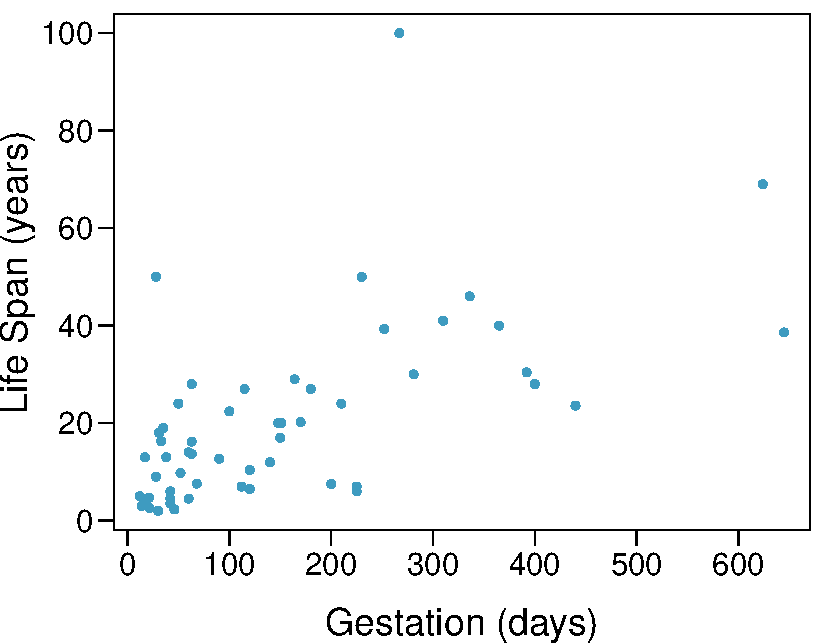
\includegraphics[width = 60mm]{01/figures/eoce/mammals/mammals_lifeSpanGest}
\end{center}
\end{minipage}
}
{
\begin{parts}
\item There is a positive association between life span and gestation, meaning that mammals with longer gestation periods tend to live longer as well.
\item The association would still be positive; if as length of gestation increases life span is expected to increase, then as life span increases, length of gestation is expected to increase as well.
\item No, they are not independent since there is a clear association between the two variables.
\end{parts}
}

% 24

\eoce{\qt{Office productivity} Office productivity is relatively low when the employees feel no stress about their work or job security. However, high levels of stress can also lead to reduced employee productivity. Sketch a plot to represent the relationship between stress and productivity and explain your reasoning.}
{
\begin{center}
\begin{minipage}[c]{0.55\textwidth}
We would expect productivity to increase as stress increases, but up to a point, after that productivity would decrease as stress continued to increase. The exact shape of your plot may have a slightly different shape for increasing then decreasing.
\end{minipage}
\begin{minipage}[c]{0.4\textwidth}
\begin{center}
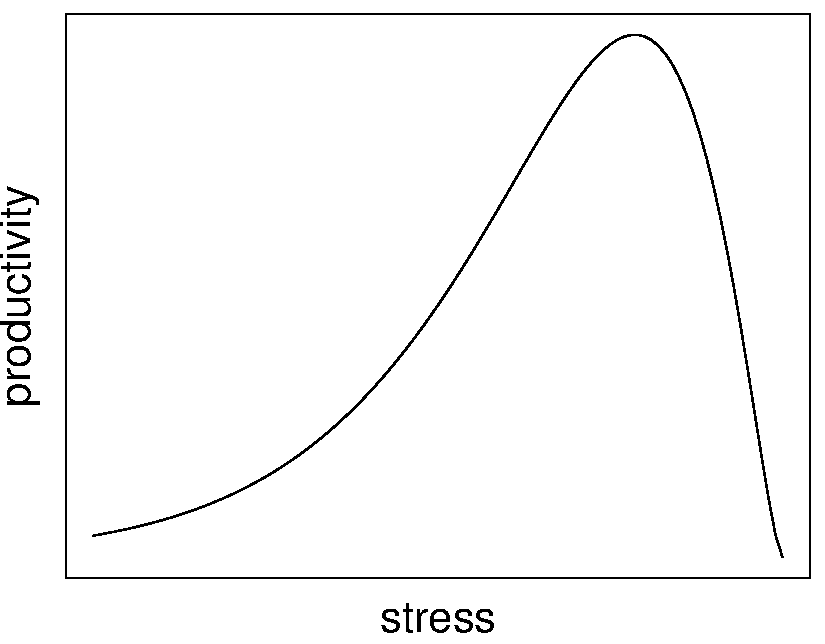
\includegraphics[width = 40mm]{01/figures/eoce/stressProductivity/stressProductivity}
\end{center}
\end{minipage}
\end{center}
}

% 25

\noindent\begin{minipage}[b]{0.55\textwidth}
\eoce{\qt{Associations} Indicate which of the plots to the right show a
\begin{parts}
\item positive association
\item negative association
\item no association
\end{parts}
Also determine if the positive and negative associations are linear or nonlinear. Each part may refer to more than one plot.\vspace{2mm}
}
{
\begin{parts}
\item (1) - linear and (3) - nonlinear
\item (4) - linear
\item (2)
\end{parts}
}
\end{minipage}
\begin{minipage}[b]{0.45\textwidth}
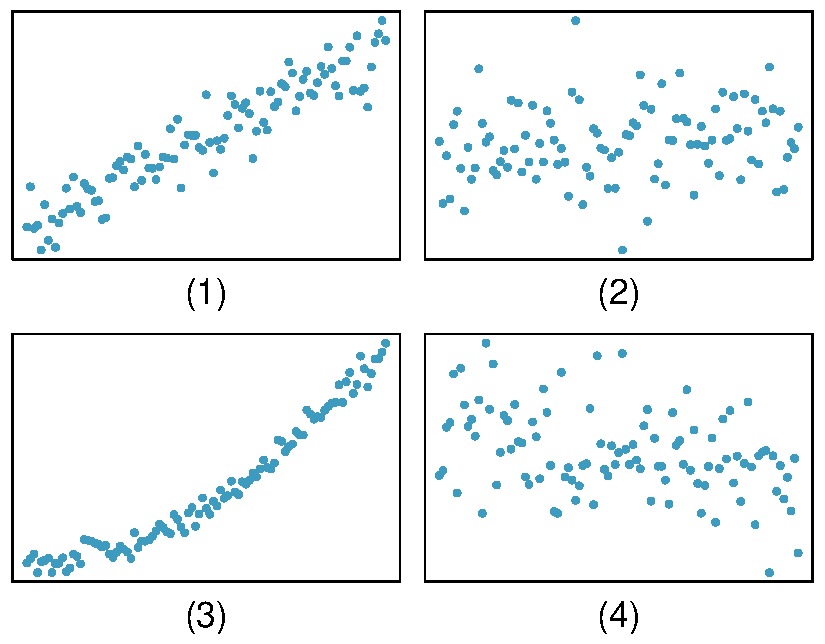
\includegraphics[width = 0.9\textwidth]{01/figures/eoce/associationPlots/associationPlots} \\
\end{minipage}

% 26

\eoce{\qt{Parameters and statistics} Identify which value represents the sample mean and which value represents the claimed population mean.
\begin{parts}
\item A recent article in a college newspaper stated that college students get an average of 5.5 hrs of sleep each night. A student who was skeptical about this value decided to conduct a survey by randomly sampling 25 students. On average, the sampled students slept 6.25 hours per night.
\item American households spent an average of about \$52 in 2007 on Halloween merchandise such as costumes, decorations and candy. To see if this number has changed, researchers conducted a new survey in 2008 on 1,500 households and found that in the average amount a household spent on Halloween was \$58.
\item The average GPA of students in 2001 at a private university was 3.37. A survey on a sample of 203 students from this university yielded an average GPA of 3.59 in Spring semester of 2012.
\end{parts}
}
{
\begin{parts}
\item Population mean (claimed by a college paper), $\mu_x = 5.5$; sample mean, $\bar{x} = 6.25$.
\item Population mean, $\mu_{2007} = 52$; sample mean, $\bar{x}_{2008} = 58$.
\item Population mean, $\mu_{2001} = 3.37$; sample mean, $\bar{x}_{2012} = 3.59$.
\end{parts}
}

% 27

\eoce{\qt{Make-up exam} In a class of 25 students, 24 of them took an exam in class and 1 student took a make-up exam the following day. The professor graded the first batch of 24 exams and found an average score of 74 points with a standard deviation of 8.9 points. The student who took the make-up the following day scored 64 points on the exam.
\begin{parts}
\item Does the new student's score increase or decrease average score?
\item What is the new average?
\item Does the new student's score increase or decrease standard deviation of the scores?
\end{parts}
}
{
\begin{parts}
\item Since the new score is smaller than the mean of the 24 previous scores, the new mean should be smaller than the old mean.
\item We are given that $ n = 24,\quad \bar{x} = 74,\quad s_x = 8.9$.
\begin{align*}
\bar{x} &= \frac{x_1 + x_2 + \dots + x_{24}}{24} = 74\\
x_1 + x_2 + \dots + x_{24} &= 74 * 24 = 1776\\
x_1 + x_2 + \dots + x_{24} + x_{25} &= 1776 + 64 = 1840\\
\bar{x}_{new} &= \frac{x_1 + x_2 + \dots+x_{24} + x_{25}}{25}=\frac{1840}{25} = 73.6
\end{align*}
\item The new score, $x_{25}$, is more than 1 standard deviation away from the previous mean, and this will tend to increase the standard deviation of the data. While possible, it is mathematically tedious to calculate the new standard deviation.
\end{parts}
}

% 28

\eoce{\qt{Days off at a mining plant} Workers at a particular mining site receive an average of 35 days paid vacation, which is lower than the national average. The manager of this plant is under pressure from a union to increase the amount of paid time off. However, he does not want to give more days off to the workers because that would be costly. Instead he decides he should fire 10 employees in such a way as to raise the average number of days off that are reported by his employees. In order to achieve this goal, should he fire employees who have the most number of days off, least number of days off, or those who have about the average number of days off?
}
{
In order to increase the average number of days off, the manager should fire any 10 employees whose average number of days off is between the minimum and the mean number of days off for the entire workforce at this plant. However, firing the 10 employees with the minimum number of days off will have the biggest impact on the average.
}

% 29

\eoce{\qt{Smoking habits of UK residents, revisited} Exercise~\ref{UKSmoking_datamatrix} introduces a data set on the smoking habits of UK residents. Below are histograms displaying the distributions of the number of cigarettes smoked on weekdays and weekends. Describe the two distributions and compare them.
\begin{center}
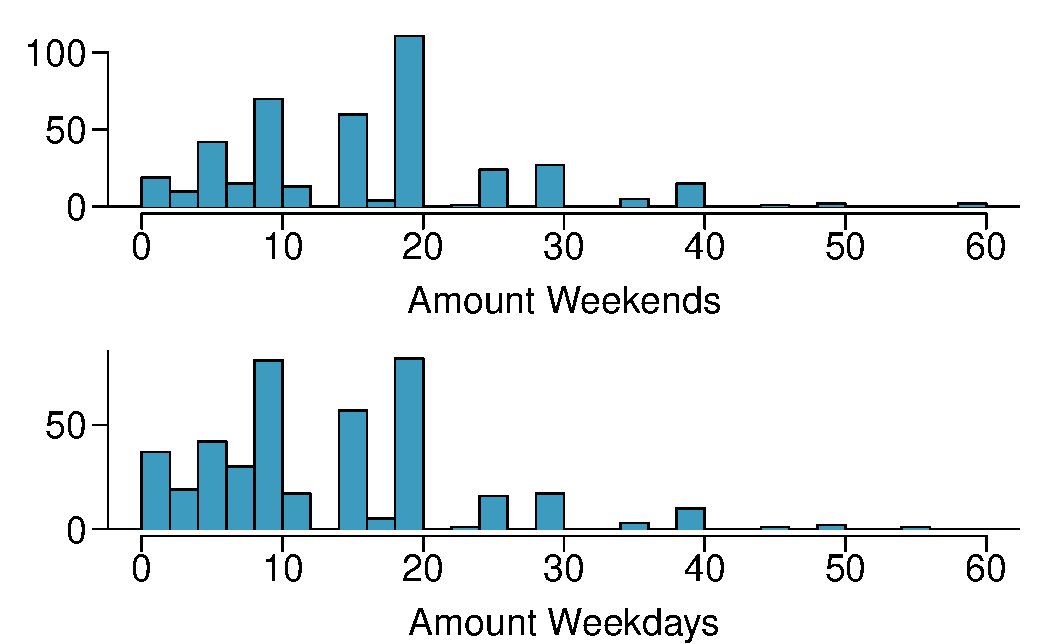
\includegraphics[width = 0.7\textwidth]{01/figures/eoce/smoking/smoking_amountHist}
\end{center}
}
{The distribution of amount of cigarettes smoked on weekends and on weekdays are both right skewed and bimodal with modes at 10 and 20 cigarettes. This may be because most people do not keep track of exactly how many cigarettes they smoke, but round their answers to half a pack (10 cigarettes) or a whole pack (20 cigarettes). The median of both distributions is between 10 and 15 cigarettes. The middle 50\% of the data (the IQR) appears to be spread equally in each group and have a width of about 10 to 15. There are potential outliers above 40 cigarettes per day, and both distributions a long right tail. We can also see that there are more respondents who smoke only a few cigarettes (0 to 5) on the weekdays, about 80 people, than on weekends, about 60 people.}\label{UKSmoking_amounts}

% 31

\eoce{\qt{Stats scores} Below are the final scores of 20 introductory statistics students.
\begin{center}
79, 83, 57, 82, 94, 83, 72, 74, 73, 71, \\
66, 89, 78, 81, 78, 81, 88, 69, 77, 79
\end{center}
Draw a histogram of these data and describe the distribution.
}
{
In order to draw a histogram we first need create a frequency distribution table.

\begin{minipage}[c]{0.4\textwidth}
\begin{center}
\begin{tabular}{cr}
Score & Frequency \\
\hline
55 - 59	& 1 \\
60 - 64	& 0 \\
65 - 69	& 2 \\
70 - 74	& 4 \\
75 - 79	& 5 \\
80 - 84	& 5 \\
85 - 89	& 2 \\
90 - 95	& 1 \\
\hline
Total & 20
\end{tabular}
\end{center}
\end{minipage}
\begin{minipage}[c]{0.35\textwidth}
\begin{center}
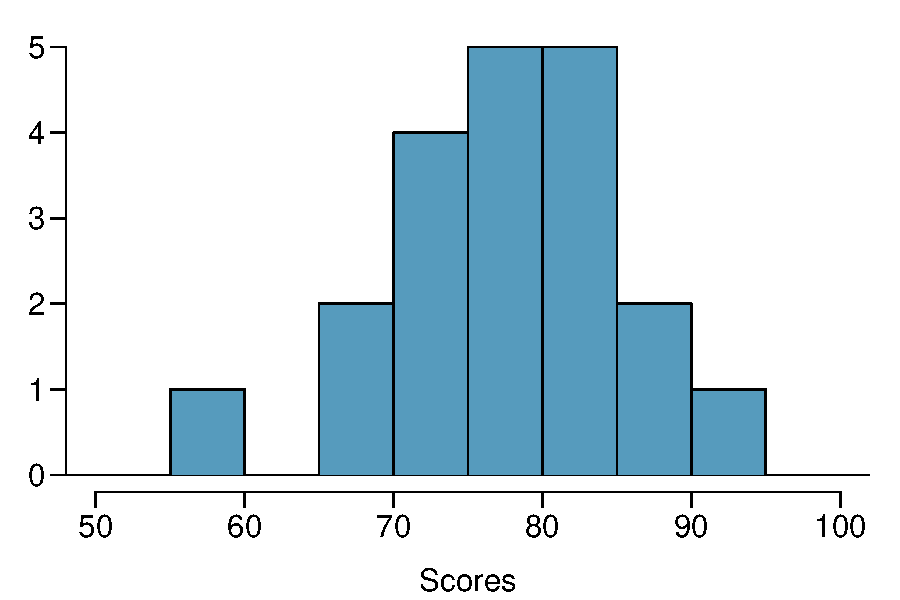
\includegraphics[height = \textwidth]{01/figures/eoce/statsFinalScores/statsFinalScores_hist} 
\end{center}
\end{minipage}

The distribution is unimodal and symmetric with a mean at 77.7 and a standard deviation of approximately 8.4. About 80\% of scores are within 10 points of the mean (between 68 and 88).
}\label{introStatsFinalScores}

% 31

\eoce{\qt{Smoking habits of UK residents, III} A random sample of 5 smokers from the data set discussed in Exercises~\ref{UKSmoking_datamatrix} and \ref{UKSmoking_amounts} is provided below.
{\footnotesize
\begin{center}
\begin{tabular}{ccccccc}
  \hline
gender & age & maritalStatus & grossIncome & smoke & amtWeekends & amtWeekdays \\ 
  \hline
Female &  51 & Married & $\pounds$2,600 to $\pounds$5,200 & Yes &  20 cig/day &  20 cig/day\\ 
  Male &  24 & Single & $\pounds$10,400 to $\pounds$15,600 & Yes &  20 cig/day&  15 cig/day\\ 
  Female &  33 & Married & $\pounds$10,400 to $\pounds$15,600 & Yes &  20 cig/day&  10 cig/day\\ 
  Female &  17 & Single & $\pounds$5,200 to $\pounds$10,400 & Yes &  20 cig/day&  15 cig/day\\ 
  Female &  76 & Widowed & $\pounds$5,200 to $\pounds$10,400 & Yes &  20 cig/day&  20 cig/day\\ 
   \hline
\end{tabular}
\end{center}
}
\begin{parts}
\item Find the mean amount of cigarettes smoked on weekdays and weekends by these 5 respondents.
\item Find the standard deviation of the amount of cigarettes smoked on weekdays and on weekends by these 5 respondents. Is the variability higher on weekends or on weekdays?
\end{parts}
}
{
\begin{parts}
\item Means are calculated below:
\begin{align*}
\bar{x}_{amtWeekends} &= \frac{20 + 20 + 20 + 20 + 20}{5} = 20 \\
\bar{x}_{amtWeekdays} &= \frac{20 + 15 + 10 + 15 + 20}{5} = 16
\end{align*}
\item Standard deviations are calculated below:
\begin{align*}
s^2_{amtWeekends} &= \frac{(20 - 20)^2 + (20 - 20)^2 + (20 - 20)^2 + (20 - 20)^2 + (20 - 20)^2}{5 - 1}  = 0 \\
s_{amtWeekends} &= \sqrt{0} = 0 \\
s^2_{amtWeekdays} &= \frac{(20 - 16)^2 + (15 - 16)^2 + (10 - 16)^2 + (15 - 16)^2 + (20 - 16)^2}{5 - 1} = 17.5 \\
s_{amtWeekdays} &= \sqrt{562.7} = 4.18 \\
\end{align*}
Standard deviation for the weekends is 0 while it is 4.18 for the weekdays. The variability of the amount of cigarettes smoked is higher on weekdays than on the weekends for this sample.
\end{parts}
}

% 32

\eoce{\qt{Factory defective rate} A factory quality control manager decides to investigate the percentage of defective items produced each day. Within a given work week (Monday through Friday) the percentage of defective items produced was 2\%, 1.4\%, 4\%, 3\%, 2.2\%.
\begin{parts}
\item Calculate the mean for these data.
\item Calculate the standard deviation for these data, showing each step in detail.
\end{parts}
}
{
\begin{parts}
\item Mean: $ \bar{x} = \frac{2 + 1.4 + 4 + 3 + 2.2}{5} = \frac{12.6}{5} = 2.52 $
\item Variance: $ s_x^2 =\frac{(2 - 2.52)^2+ (1.4 - 2.52)^2 + (4 - 2.52)^2 + (3 - 2.52)^2 + (2.2 - 2.52)^2}{5 - 1} = \frac{4.048}{4} = 1.012 $ \\
Standard deviation: $s_x = \sqrt{1.012} = 1.006 $
\end{parts}
}

% 33

\eoce{\qt{Medians and IQRs} Compare distributions (1) and (2) based on their medians and IQRs. You do not need to calculate these statistics, simply state how the medians and IQRs compare. Make sure to explain your reasoning. 
\begin{multicols}{2}
\begin{parts}
\item (1) 3, 5, 6, 7, 9 \\
(2) 3, 5, 6, 7, 20
\item (1) 3, 5, 6, 7, 9 \\
(2) 3, 5, 8, 7, 9
\item (1) 1, 2, 3, 4, 5 \\
(2) 6, 7, 8, 9, 10
\item (1) 0, 10, 50, 60, 100 \\
(2) 0, 100, 500, 600, 1000
\end{parts}
\end{multicols}
}
{
\begin{parts}
\item Both distributions have the same median, 6, and the same IQR. The only difference between the two distributions is the maximum, which does not affect either of these statistics.
\item Both distributions have the same IQR, but distribution (2) has a slightly higher median, $8 > 5$.
\item Distribution (2) has a higher median, $8 > 3$, but the variability in the distributions is the same so their IQRs will be equal as well.
\item Distribution (2) has a higher median, $500 > 50$, and a much wider range which, in this case, also yields a much wider IQR.
\end{parts}
}

% 34

\eoce{\qt{Means and SDs} Compare distributions (1) and (2) based on their means and standard deviations. You do not need to calculate these statistics, simply state how the means and the standard deviations compare. Make sure to explain your reasoning. \textit{Hint:} It may be useful to sketch dot plots of the distributions.
\begin{multicols}{2}
\begin{parts}
\item (1) 3, 5, 5, 5, 8, 11, 11, 11, 13 \\
(2) 3, 5, 5, 5, 8, 11, 11, 11, 20 \\
\item (1) -20, 0, 0, 0, 15, 25, 30, 30 \\
(2) -40, 0, 0, 0, 15, 25, 30, 30
\item (1) 0, 2, 4, 6, 8, 10 \\
(2) 20, 22, 24, 26, 28, 30
\item (1) 100, 200, 300, 400, 500 \\
(2) 0, 50, 300, 550, 600
\end{parts}
\end{multicols}
}
{
\begin{parts}
\item Distribution (2) has a higher mean since $20 > 8$, and a higher standard deviation since 20 is much further from the rest of the data than 8.
\item Distribution (1) has a higher mean since $-20 > -40$, and distribution (2) has a higher standard deviation since -40 is farther away from the rest of the data than -20.
\item Distribution (2) has a higher mean since all values in this distribution are higher than those in distribution (1), but both distribution have the same standard deviation since they are equally variable around their respective means.
\item Both distributions have the same mean since they're both centered at 300, but distribution (2) has a higher standard deviation since the observations are farther from the mean than in distribution (1).
\end{parts}
}

% 35

\eoce{\qt{Box plot} Below is the five number summary for the data given in Exercise~\ref{introStatsFinalScores}. Create a box plot of the data based on these values.
\begin{center}
\renewcommand\arraystretch{1.5}
\begin{tabular}{ccccc}
Min	& Q1	& Q2 (Median)	& Q3	& Max \\
\hline
57	& 72.5	& 78.5	& 82.5	& 94 \\
\end{tabular}
\end{center}
}
{
\begin{itemize}
\item The box goes from Q1 (72.5) to Q3 (82.5), the line inside the box is the median (78.5).
\item Below is how we determine where the whiskers go and check for observations that should be individually labeled:
\begin{align*}
\text{IQR} &= Q3 - Q1 = 82.5 - 72.5 = 10 \\
\text{Upper Fence} &= Q3 + 1.5 * IQR = 82.5 + 1.5 * 10 = 97.5 \\
\text{Lower Fence} &= Q1 - 1.5 * IQR = 72.5 - 1.5 * 10 = 57.5
\end{align*}
\end{itemize}

\begin{center}
\begin{minipage}[c]{0.47\textwidth}
\begin{itemize}
\item Any point above the UF should be labeled an outlier: none \\
Any point below the LF should be labeled an outlier: 57
\item Since there is an observation that falls below the LF, the lower whisker goes till the last point above the LF: 66 \\
Since no observations extend beyond the UF, the upper whisker goes till the maximum: 94
\end{itemize}
\end{minipage}
\begin{minipage}[c]{0.45\textwidth}
\hspace{10mm} 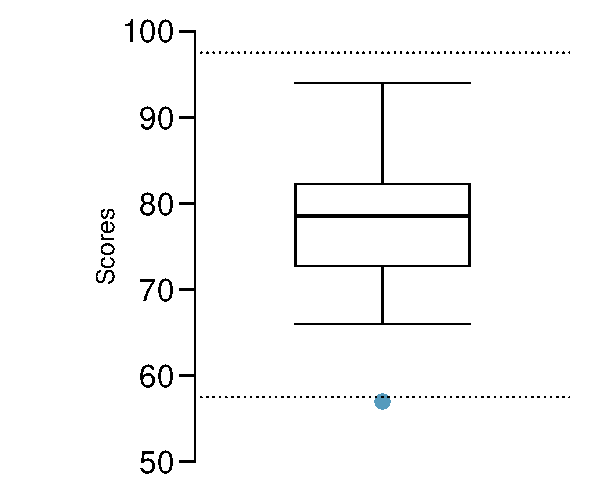
\includegraphics[width = 60mm]{01/figures/eoce/statsFinalScores/statsFinalScores_box}
\end{minipage}
\end{center}
}

% 36

\eoce{\qt{Infant mortality} The infant mortality rate is defined as the number of deaths of infants under one year old in a given year per 1,000 live births in the same year. This rate is often used as an indicator of the level of health in a country. The relative frequency histogram below shows the distribution of the infant death rates in 2012 for 222 countries as provided by the CIA Factbook. \footfullcite{data:ciaFactBookInfMort:2012}

\noindent\begin{minipage}[c]{0.45\textwidth}
\begin{parts}
\item Estimate Q1, the median, and Q3 from the histogram.
\item Would you expect the mean of this data set to be smaller or larger than the median? Explain your reasoning.
\end{parts}
\vspace{2cm}
\end{minipage}
\begin{minipage}[c]{0.5\textwidth}
\begin{center}
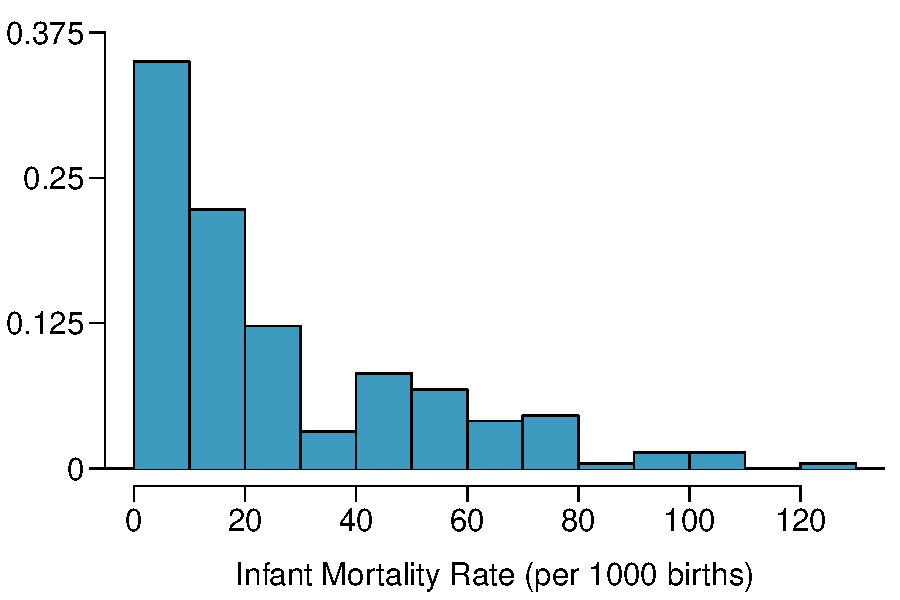
\includegraphics[width = 0.9\textwidth]{01/figures/eoce/country/country_infMort}
\end{center}
\end{minipage}
}
{
\begin{parts}
\setlength{\itemsep}{0mm}
\item Since about 35\% of the data is in the first bar this is where Q1 is, between 0 and 10. The median is in the second bar, between 10 and 20. Q3 is in the third bar, between 40 an 50.
\item The distribution is right-skewed, so the long tail will pull the mean above the median.
\end{parts}
}

% 37

\eoce{\qt{Matching histograms and box plots} Describe the distribution in the histograms below and match them to the box plots. \\
\begin{center}
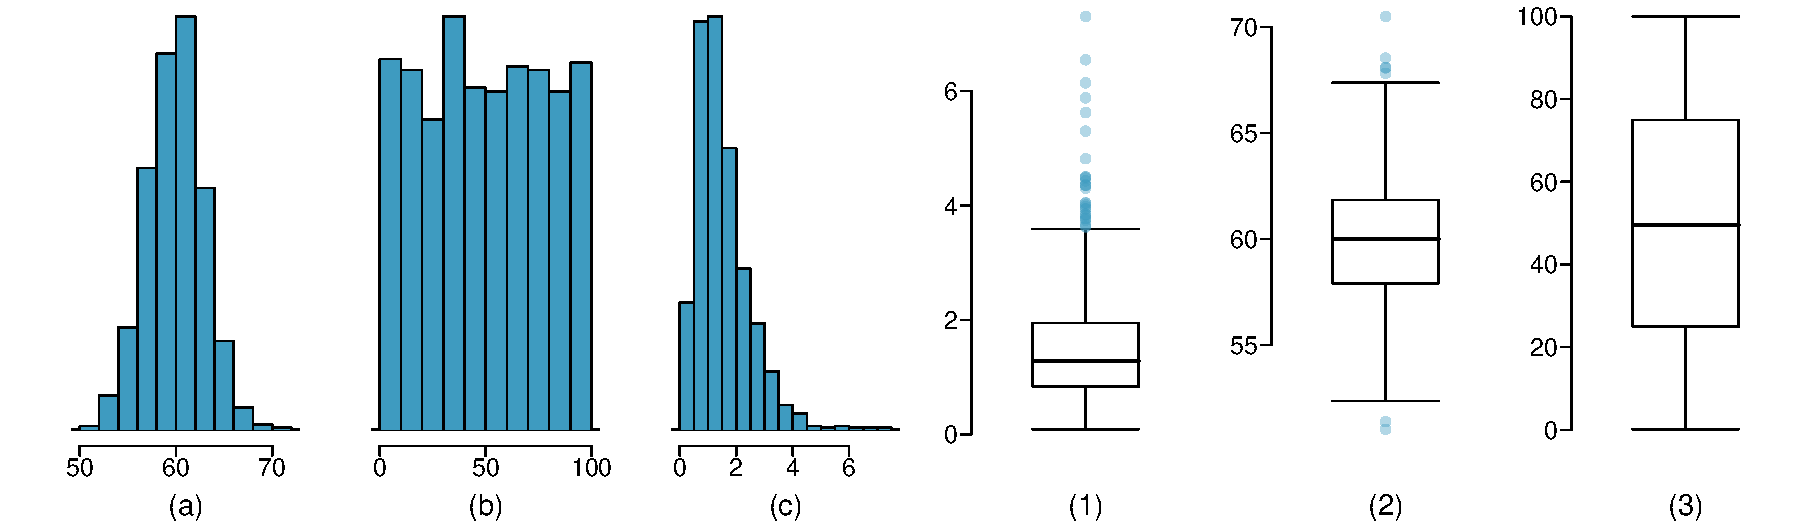
\includegraphics[width =\textwidth]{01/figures/eoce/histBoxMatch/histBoxMatch}
\end{center}
}
{
\begin{parts}
\item The distribution is unimodal and symmetric, and about 95\% of the data falls within about 7 units of the center, so the standard deviation will be about 3 or 4. This matches box plot (2).
\item The distribution is uniform and values range from 0 to 100. This matches box plot (3) which shows a symmetric distribution in this range. Also, each 25\% chunk of the box plot has about the same width and there are no suspected outliers.
\item The distribution is unimodal and right skewed with a median between 1 and 2. 25th and 75th percentile are near 1 and 2, so the IQR is roughly 1. This matches box plot (1).
\end{parts}
}

% 38

\eoce{\qt{Air quality} Daily air quality is measured by the air quality index (AQI) reported by the Environmental Protection Agency. This index tells you how clean or polluted your air is, and what associated health effects might be a concern for you. The index is calculated for five major air pollutants regulated by the Clean Air Act, one of which is particulate matter. Values of this index range from 0 to 300 and a higher value indicates lower air quality. AQI was reported for a sample of 91 days in 2011 in Durham, NC. The relative frequency histogram below shows the distribution of the AQI values on these days. \footfullcite{data:durhamAQI:2011}
\begin{center}
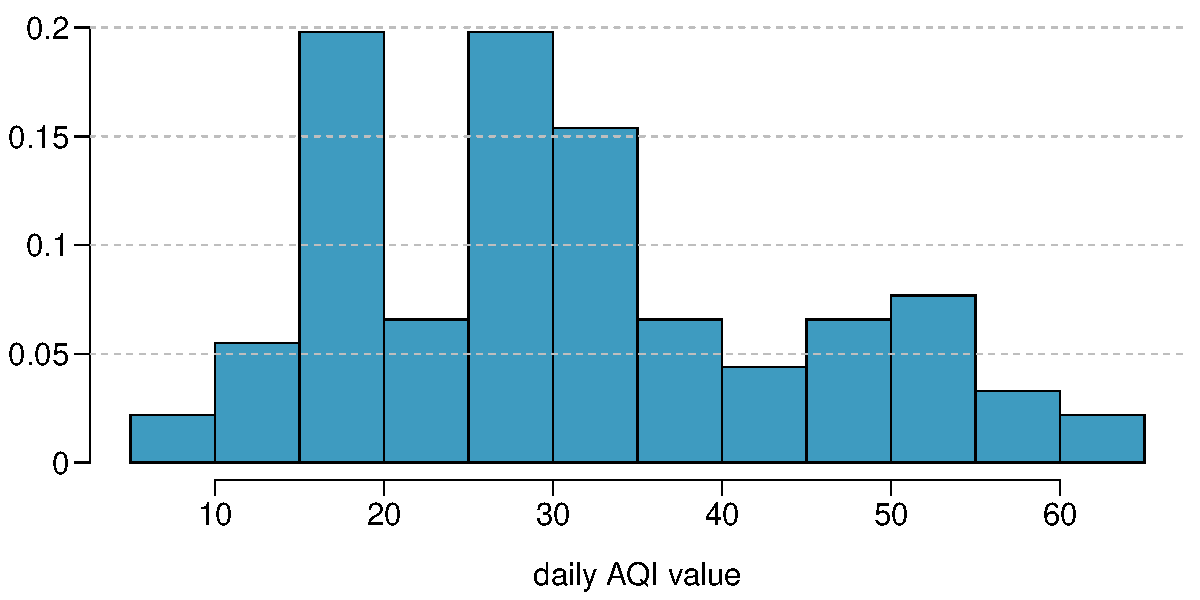
\includegraphics[width = 0.65\textwidth]{01/figures/eoce/durhamAQI/durhamAQI_hist} 
\end{center}
\begin{parts}
\item Estimate the median AQI value of this sample.
\item Would you expect the mean AQI value of this sample to be higher or lower than the median? Explain your reasoning.
\item Approximate Q1, Q3, and IQR of the distribution.
%\item Would any of the days in this sample be considered to have an unusually low or high AQI? Explain your reasoning.
\end{parts}
}
{
\begin{parts}
\item The median is the 50\% of the distribution, which is between 25 and 30.
\begin{center}
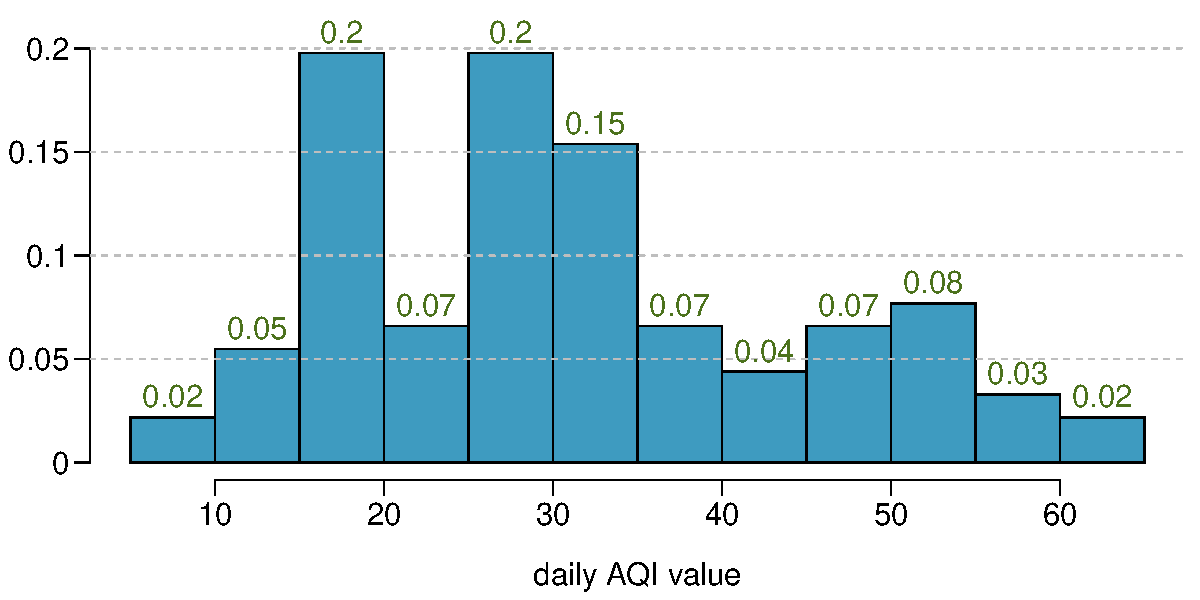
\includegraphics[width = 0.65\textwidth]{01/figures/eoce/durhamAQI/durhamAQI_histSoln} 
\end{center}
\item Since the distribution is right skewed the mean is higher than the median.
\item Q1: between 15 and 20 \\
Q3: between 35 and 40 \\
IQR: about 20
%\item Values that are considered to be unusually low or high lie more than 1.5$\times$IQR away from the quartiles. \\
%Upper fence: Q3 + 1.5 $\times$ IQR =  $37.5 + 1.5 \times 20 = 67.5$ \\
%Lower fence: Q1 - 1.5 $\times$ IQR =  $17.5 + 1.5 \times 20 =  -12.5$ \\
%The lowest AQI recorded is not lower than 5 and the highest AQI recorded is not higher than 65, which are both within the fences. Therefore none of the days in this sample would be considered to have an unusually low or high AQI.
\end{parts}
}\label{durhamAQI}

% 39

\eoce{\qt{Histograms and box plots} Compare the two plots below. What characteristics of the distribution are apparent in the histogram and not in the box plot? What characteristics are apparent in the box plot but not in the histogram?
\begin{center}
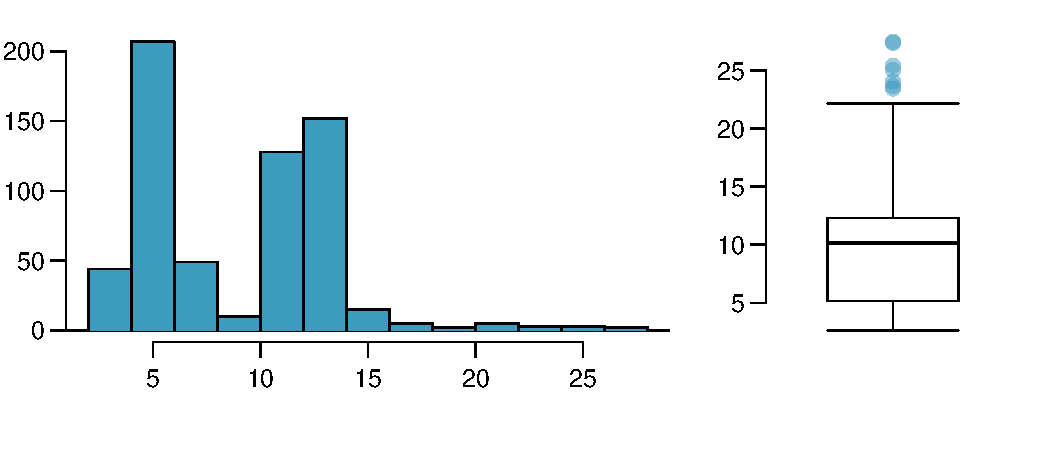
\includegraphics[width = 0.8\textwidth]{01/figures/eoce/bimodalHistBox/bimodalHistBox}
\end{center}
}
{
The histogram shows that the distribution is bimodal while this is not apparent in the box plot. On the other handthe box plot makes it easy to identify and examine individual observations that may be outliers whereas looking at the histogram it is difficult to tell if the higher values are outliers or not.
}

% 40

\eoce{\qt{Marathon winners} The histogram and the box plot below (left) shows the distribution of finishing times for male and female winners of the New York Marathon between 1980 and 1999. The figure on the right provides box plots of these data stratified by gender. \\
$\:$ \\
\begin{center}
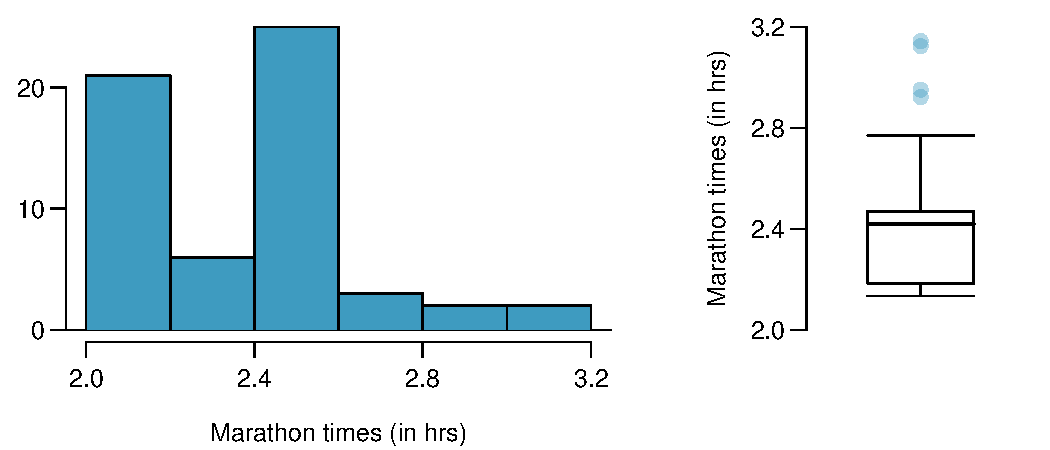
\includegraphics[width=0.5\textwidth]{01/figures/eoce/marathon/marathon_histBox}
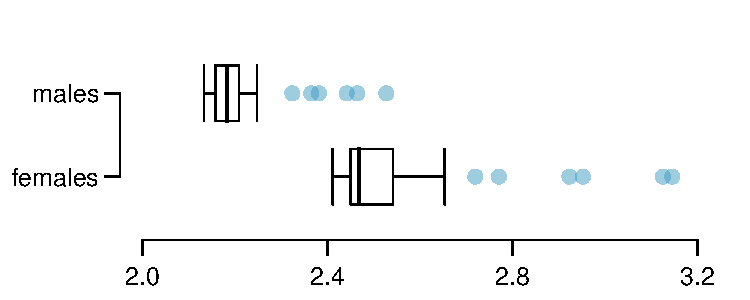
\includegraphics[width=0.49\textwidth]{01/figures/eoce/marathon/marathon_genderBox}
\end{center}
\begin{parts}
\item What features of the distribution are apparent in the histogram and not the box plot? What features are apparent in this box plot but not in the histogram?
\item What may be the reason for the bimodal distribution? Explain.
\item Compare the distribution of marathon times for men and women based on the box plot shown on the right.
\item The time series plot shown below is another way to look at these data. Describe any apparent trends in the plot and comment on whether or not these trends are apparent in the histogram and/or the box plot.
\begin{center}
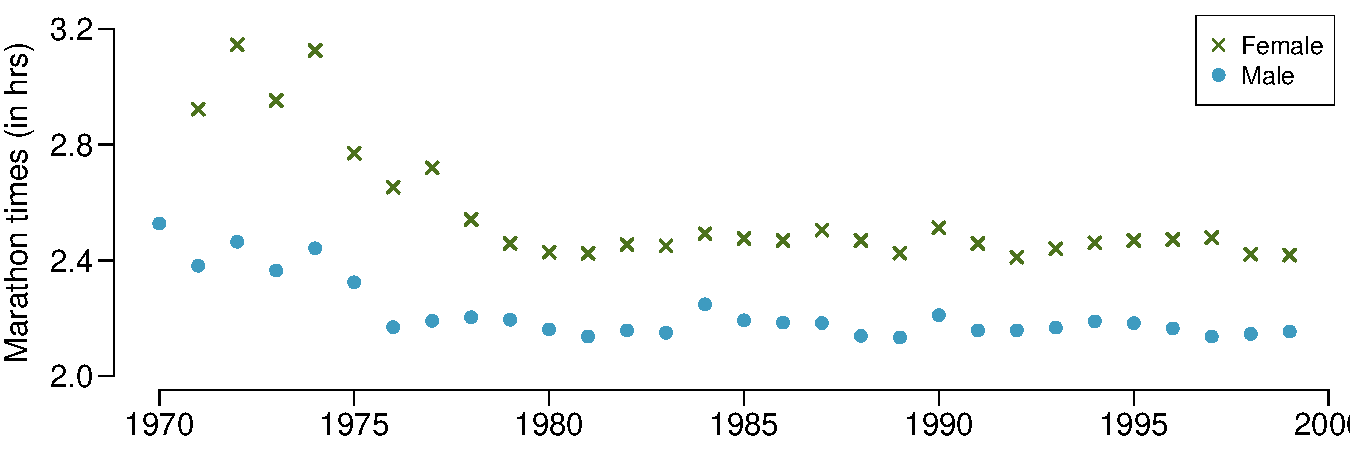
\includegraphics[width=0.85\textwidth]{01/figures/eoce/marathon/marathon_genderTimeSeries} \\
\end{center}
\end{parts}
}
{
\begin{parts}
\setlength{\itemsep}{0mm}
\item From the histogram we can see the the distribution is bimodal. In the box plot the more extreme observations, many of which could be considered outliers, are easier to identify.
\item Gender may be the reason, it is likely that men and women have different average marathon times.
\item The median marathon time for men is about 2.2 hrs while it is about 2.5 hrs for women; therefore, men are faster on average. The minimum marathon time for men is about 2.1 hrs whereas it is about 2.4 hrs for women. The maximum marathon time for men is about 2.5 hrs for men whereas it is about 3.1 hrs for women. Both distributions have apparent outliers on the high end.
\item It appears that marathon times decreased greatly between 1970-1975 and remained somewhat steady thereafter. Males consistently had shorter marathon times than females throughout the years. From the box plots of males and females, we could tell that males ran faster ``on average", however, we could not tell that the winning male time for each year was better than the winning female time. We also could not tell from the histogram or the box plot that marathon times have been decreasing for males and females throughout the years.
\end{parts}
}\label{NYMarathon}

% 41

\eoce{\qt{Robust statistics} The first histogram below shows the distribution of the yearly incomes of 40 patrons at a college coffee shop. Suppose two new people walk into the coffee shop: one making \$225,000 and the other \$250,000. The second histogram shows the new income distribution. Summary statistics are also provided. \\
\begin{minipage}[c]{0.59\textwidth}
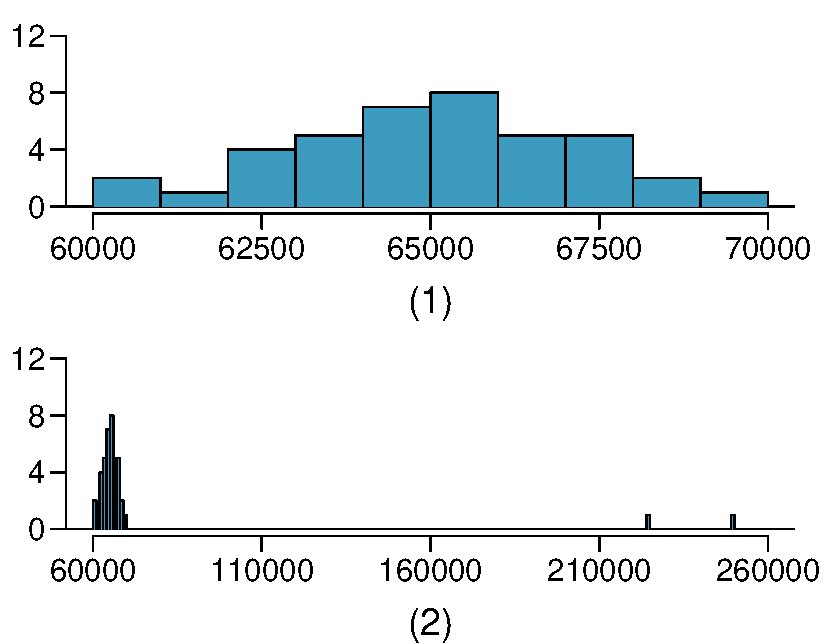
\includegraphics[width=\textwidth]{01/figures/eoce/salary/salary}
\end{minipage}
\begin{minipage}[c]{0.4\textwidth}
\begin{center}
\begin{tabular}{rrr}
  \hline
 & (1) & (2) \\ 
  \hline
n & 40 & 42 \\ 
  Min. & 60,680 & 60,680 \\ 
  1st Qu. & 63,620 & 63,710 \\ 
  Median & 65,240 & 65,350 \\ 
  Mean & 65,090 & 73,300 \\ 
  3rd Qu. & 66,160 & 66,540 \\ 
  Max. & 69,890 & 250,000 \\ 
  SD & 2,122 & 3,7321 \\ 
   \hline
\end{tabular}
\end{center}
\end{minipage}
\begin{parts}
\item Would the mean or the median best represent what we might think of as a typical income for the 42 patrons at this coffee shop? What does this say about the robustness of the two measures?
\item Would the standard deviation or the IQR best represent the amount of variability in the incomes of the 42 patrons at this coffee shop? What does this say about the robustness of the two measures?
\end{parts}
}
{
\begin{parts}
\item The median is a much better measure of the typical amount earned by these 42 people. The mean is much higher than the income of 40 of the 42 people. This is because the mean is an arithmetic average and gets affected by the two extreme observations. The median does not get effected as much since it is robust to outliers.
\item The IQR  is a much better measure of variability in the amounts earned by nearly all of the 42 people. The standard deviation gets affected greatly by the two high salaries, but the IQR is robust to these extreme observations.
\end{parts}
}

% 42

\eoce{\qt{Distributions and appropriate statistics} For each of the following, describe whether you expect the distribution to be symmetric, right skewed or left skewed. Also specify whether the mean or median would best represent the typical observation in the data, and whether the variability of observations would be best represented using the standard deviation or IQR to measure the spread.
\begin{parts}
\item Housing prices in a country where 25\% of the houses cost below \$350,000, 50\% of the houses cost below \$450,000, 75\% of the houses cost below \$1,000,000 and there are a meaningful number of houses selling at over \$6,000,000.
\item Housing prices in a country where 25\% of the houses cost below \$300,000, 50\% of the houses cost below \$600,000, 75\% of the houses cost below \$900,000 and very few houses sell at over \$1,200,000.
\item Number of alcoholic drinks consumed by college students in a given week.
\item Annual salaries of the employees of a Fortune 500 company.
\end{parts}
}
{
\begin{parts}
\item The distribution is right skewed with potential outliers on the positive end, therefore the median and the IQR are preferable measures of center and spread.
\item The distribution is somewhat symmetric and has few, if any, extreme observations, therefore the mean and the standard deviation are preferable measures of center and spread.
\item The distribution would be right skewed. There would be some students who did not consume any alcohol, but this is the minimum since students cannot consume fewer than 0 drinks. There would be a few students who consume many more drinks than their peers, giving the distribution a long right tail. Due to the skew, the median and IQR would be preferable measures of center and spread.
\item The distribution would be right skewed. Most employees would make something on the order of the median salary, but we would anticipate upper management makes much more. The distribution would have a long right tail, and the median and the IQR would be preferable measures of center or spread.
\end{parts}
}

% 43

\eoce{The histogram below shows the distribution of mean travel time to work in 3,143 counties in the US in 2010. Describe the distribution and comment on whether or not log transformation may be necessary in further analysis of these data.
\begin{center}
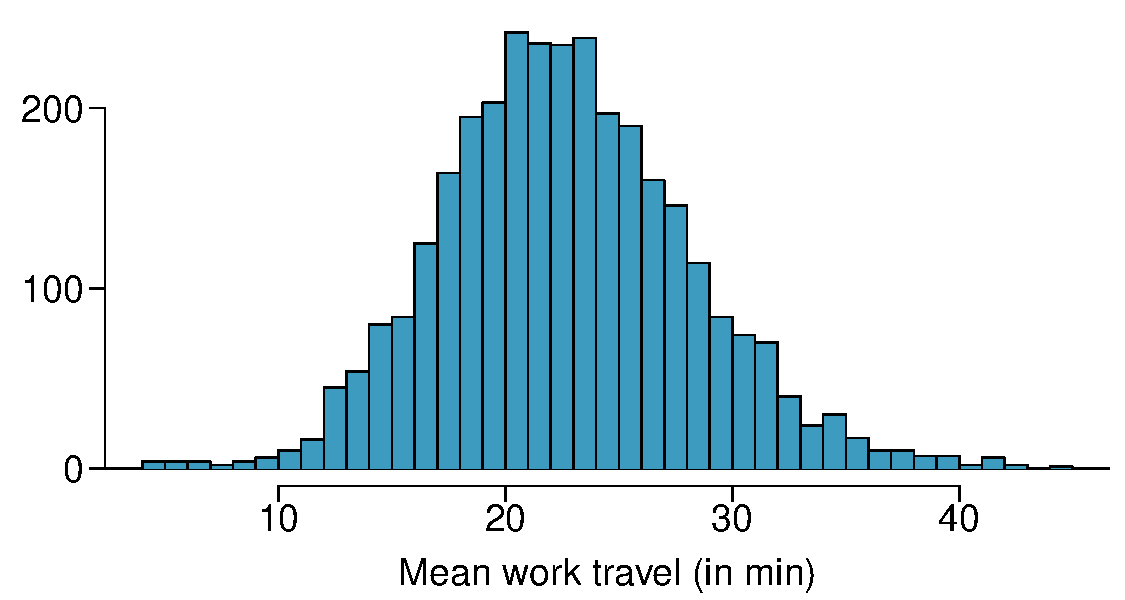
\includegraphics[width=0.5\textwidth]{01/figures/eoce/county/county_workTravelHist}
\end{center}
}
{
The distribution is unimodal and symmetric with mean of approximately 25 minutes and a standard deviation of roughly 5 minutes. There does not appear to be any counties with unusually high or low mean travel times. Since the distribution is already unimodal and symmetric, a log transformation is not necessary.
}\label{workTravel}

% 44

\eoce{The histogram below shows the distribution of percentage of population that is Hispanic in 3,143 counties in the US in 2010. Also shown is a histogram of logs of these values. Describe the distribution of percentage of population that is Hispanic and comment on why we might want to use log-transformed values in analyzing or modeling these data.
\begin{center}
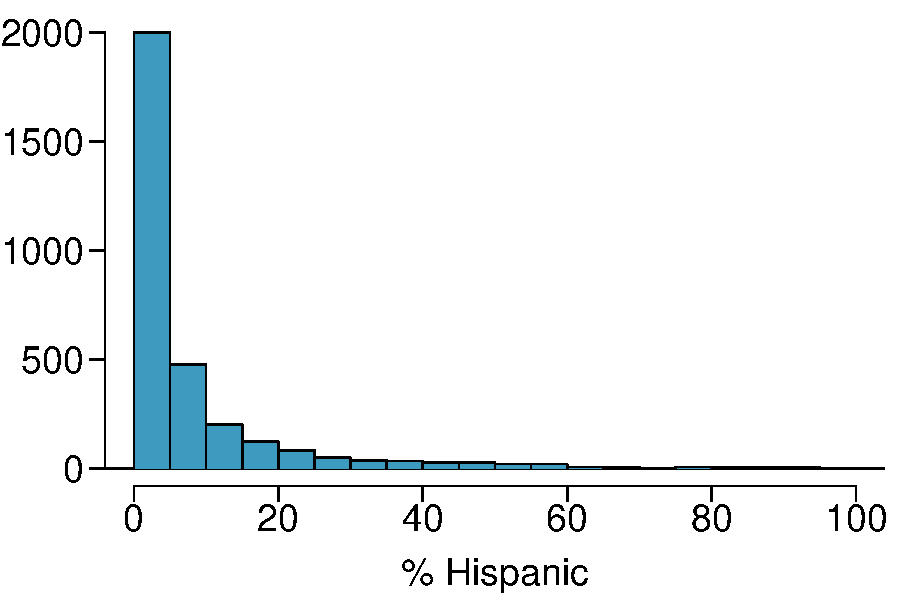
\includegraphics[width=0.49\textwidth]{01/figures/eoce/county/county_hispHist}
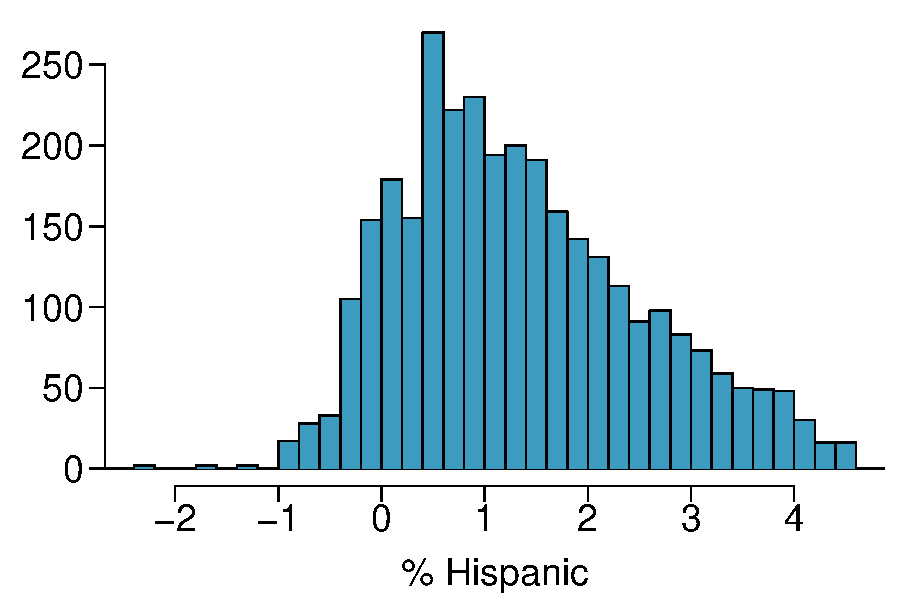
\includegraphics[width=0.49\textwidth]{01/figures/eoce/county/county_hispHistLog}
\end{center}
}
{
The distribution of percentage of population that is Hispanic is extremely right skewed with majority of counties with less than 10\% Hispanic residents. However there are a few counties that have more than 90\% Hispanic population. It might be preferable to, in certain analyses, to use the log-transformed values since this distribution is much less skewed.}\label{hispHist}


% 45

\eoce{Exercise~\ref{workTravel} displays histograms of mean travel time to work in 3,143 counties in the US in 2010. Shown below is a spatial map of these data. 
\begin{center}
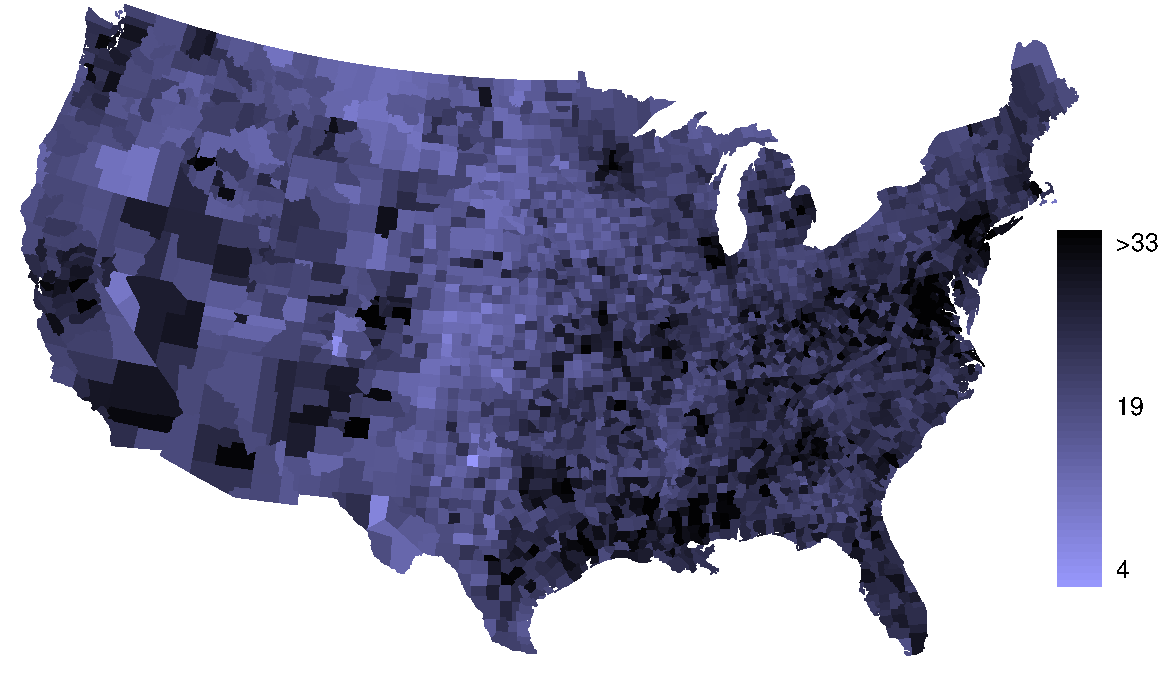
\includegraphics[width=\textwidth]{01/figures/eoce/county/county_workTravelMap}
\end{center}
}
{There are pockets of longer travel time around DC, Southeastern NY, Chicago, Minneapolis, Los Angeles, and many other big cities. There is also a large section of shorter average commute times that seems to overlap with farmland in the Midwest. Since many farmers' homes are adjacent to their farmland, their commute would be 0 minutes, which may explain why the average commute time for these counties is relatively low.}

% 46

\eoce{Exercise~\ref{hispHist} displays histograms of the distribution of percentage of population that is Hispanic in 3,143 counties in the US in 2010. Shown below is a spatial map of these data. 
\begin{center}
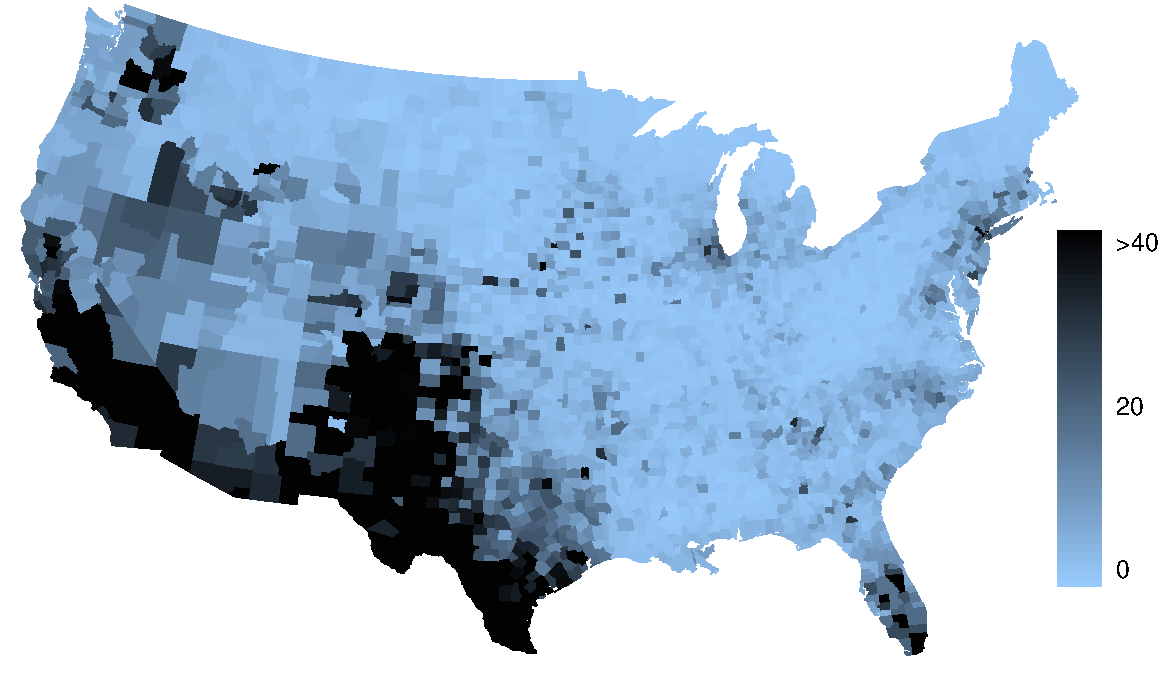
\includegraphics[width=\textwidth]{01/figures/eoce/county/county_hispMap}
\end{center}
\begin{parts}
\item What features of this distribution that are apparent in the map but not in the histogram? 
\item What features are apparent in the histogram but not the map? 
\item Is one visualization more appropriate or helpful than the other? Explain your reasoning.
\end{parts}
}
{
\begin{parts}
\item The map reveals that counties with higher proportions of Hispanic residents are clustered along the Southwest border, all of New Mexico, a large swath of Southwest Texas, the bottom two-thirds of California, and in Southern Florida.
\item In the map all counties with more than 40\% of Hispanic residents are indicated by the darker shading, so it is impossible to discern the how high Hispanic percentages go. The histogram reveals that there are counties with over 90\% Hispanic residents. The histogram is also useful for estimating measures of center and spread.
\item Both visualizations are useful, but if we could only examine one, we should examine the map since it explicitly ties geographic data to each county's percentage.
\end{parts}
}

%%%%%%%%%%%%%%%%%%%%%%%%%%%%%%%%%%%%%

\subsection{Considering categorical data}

%%%%%%%%%%%%%%%%%%%%%%%%%%%%%%%%%%%%%

% 47

\eoce{\qt{Antibiotic use in children} The bar plot and the pie chart below show the distribution of pre-existing medical conditions of children involved in a study on the optimal duration of antibiotic use in treatment of tracheitis (upper respiratory infection).
\begin{parts}
\item What features are apparent in the bar plot but not in the pie chart?
\item What features are apparent in the pie chart but not in the bar plot?
\item Which graph would you prefer to use for displaying these categorical data?
\end{parts}
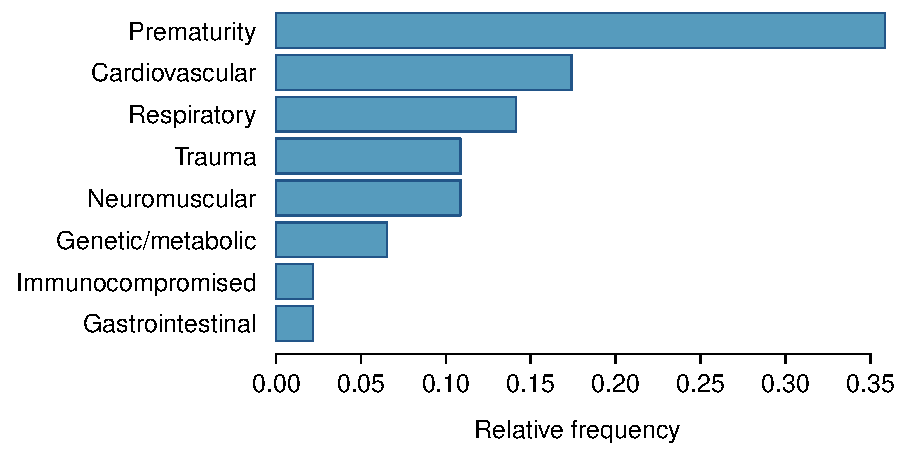
\includegraphics[width = 0.6\textwidth]{01/figures/eoce/tracheitis/tracheitis_bar}
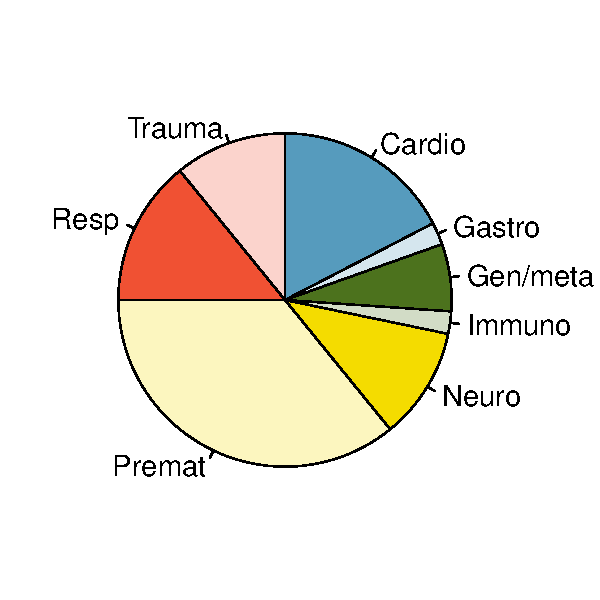
\includegraphics[width = 0.35\textwidth]{01/figures/eoce/tracheitis/tracheitis_pie}
}
{
\begin{parts}
\item As well as the order of the categories, we can also see the relative frequencies in the bar plot. These proportions are not readily available in the pie chart.
\item There are no features that are apparent in the pie chart but not in the bar plot.
\item We usually prefer to use a bar plot as we can also see the relative frequencies of the categories in this graph.
\end{parts}
}

% 48

\eoce{\qt{Views on immigration} 910 randomly sampled registered voters from Tampa, FL were asked if they thought workers who have illegally entered the US should be (i) allowed to keep their jobs and apply for US citizenship, (ii) allowed to keep their jobs as temporary guest workers but not allowed to apply for US citizenship, or (iii) lose their jobs and have to leave the country. The results of the survey by political ideology is shown below.\footfullcite{survey:immigFL:2012}
\begin{center}
\begin{tabular}{l l  c c c c}
				&		& \multicolumn{3}{c}{\textit{Political ideology}} \\
\cline{3-5}
				& & Conservative	& Moderate	& Liberal 	& Total \\
\cline{2-6}
& (i) Apply for citizenship	& 57			& 120		& 101	& 278 \\
& (ii) Guest worker		& 121		& 113		& 28		& 262 \\
\raisebox{1.5ex}[0pt]{\emph{Response}} &(iii) Leave the country	& 179		& 126		& 45		& 350 \\ 
& (iv) Not sure			& 15			& 4			& 1		& 20\\
\cline{2-6}
& Total				& 372		& 363		& 175	& 910
\end{tabular}
\end{center}
\begin{parts}
\item What is percent of these Tampa, FL voters identify themselves as conservatives?
\item What is percent of these Tampa, FL voters are in favor of the citizenship option?
\item What is percent of these Tampa, FL voters identify themselves as conservatives and are in favor of the citizenship option?
\item What is percent of these Tampa, FL voters who identify themselves as conservatives are also in favor of the citizenship option? What percent of moderates and liberal share this view?
\item Do political ideology and views on immigration appear to be independent? Explain your reasoning.
\end{parts}
}
{
\begin{parts}
\item $\frac{372}{910} = 0.41 \rightarrow 41\%$
\item $\frac{278}{910} = 0.31 \rightarrow 31\%$
\item $\frac{57}{910} = 0.06 \rightarrow 6\%$
\item Conservatives: $\frac{57}{372} = 0.15 \rightarrow 15\%$ \\
Moderates: $\frac{120}{363} = 0.33 \rightarrow 33\%$ \\
Liberals: $\frac{101}{175} = 0.58 \rightarrow 58\%$
\item The percentages of Tampa, FL conservatives, moderates, and liberals who are in favor of illegal immigrants working in the US staying and applying for citizenship are quite different from one another. Therefore, the two variables appear to be dependent.
\end{parts}
}\label{immigration}

% 49

\noindent\begin{minipage}[c]{0.5\textwidth}
\eoce{\qt{Views on the DREAM Act} The same survey from Exercise~\ref{immigration} also asked respondents if they support the DREAM Act, a proposed law which would provide a path to citizenship for people brought illegally to the US as children. Based on the mosaic plot shown on the right, are views on the DREAM Act and political ideology independent.}
{
The vertical locations at which the ideological groups break into the Yes, No, and Not Sure categories differ, which indicates the variables are dependent.}
\end{minipage}
\begin{minipage}[c]{0.5\textwidth}
\begin{center}
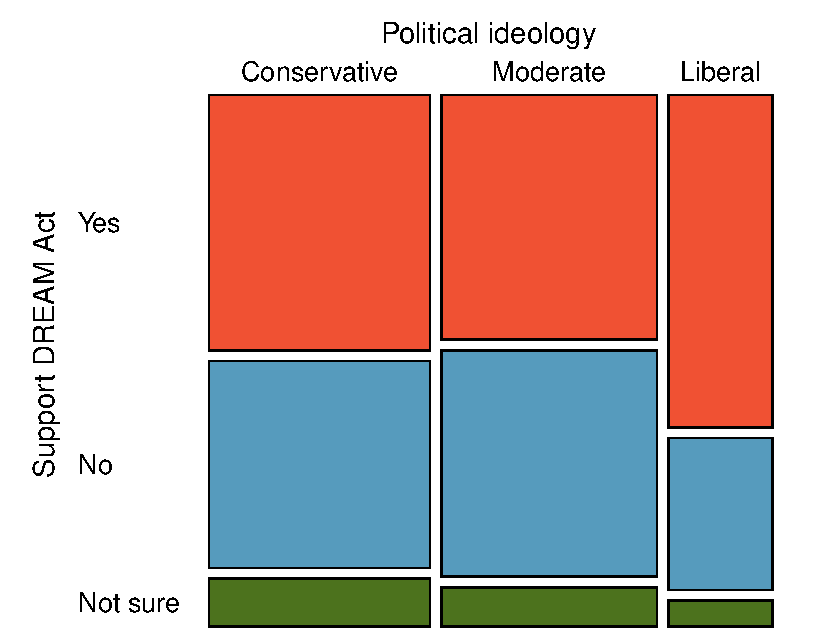
\includegraphics[width = \textwidth]{01/figures/eoce/dreamAct/dreamAct_mosaic}
\end{center}
\end{minipage}

% 50

\eoce{\qt{Heart transplants} The Stanford University Heart Transplant Study was conducted to determine whether an experimental heart transplant program increased lifespan. Each patient entering the program was designated an official heart transplant candidate, meaning that he was gravely ill and would most likely benefit from a new heart. Some patients got a transplant and some did not. The variable \texttt{transplant} indicates what group the patients were in; patients in the treatment group got a transplant and those in the control group did not. Another variable called \texttt{survived} was used to indicate whether or not the patient was alive at the end of the study. \footfullcite{Turnbull+Brown+Hu:1974}
\begin{parts}
\item Based on the mosaic plot, is survival independent of whether or not the patient got a transplant? Explain your reasoning.
\item What do the box plots below suggest about the efficacy (effectiveness) of transplants?
\end{parts}
\begin{minipage}[c]{0.5\textwidth}
\begin{center}
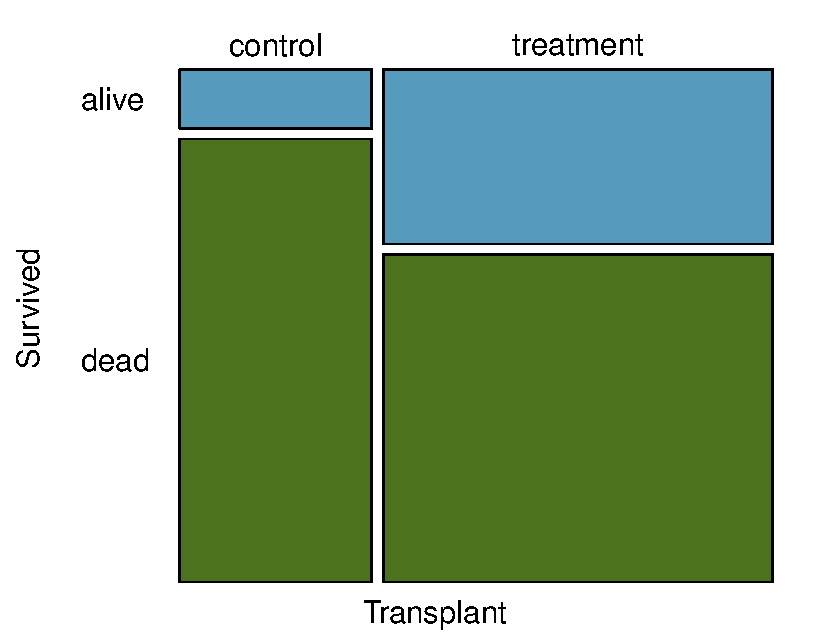
\includegraphics[width= 0.95\textwidth]{01/figures/eoce/heartTr/heartTr_SurvTrMosaic}
\end{center}
\end{minipage}
\begin{minipage}[c]{0.5\textwidth}
\begin{center}
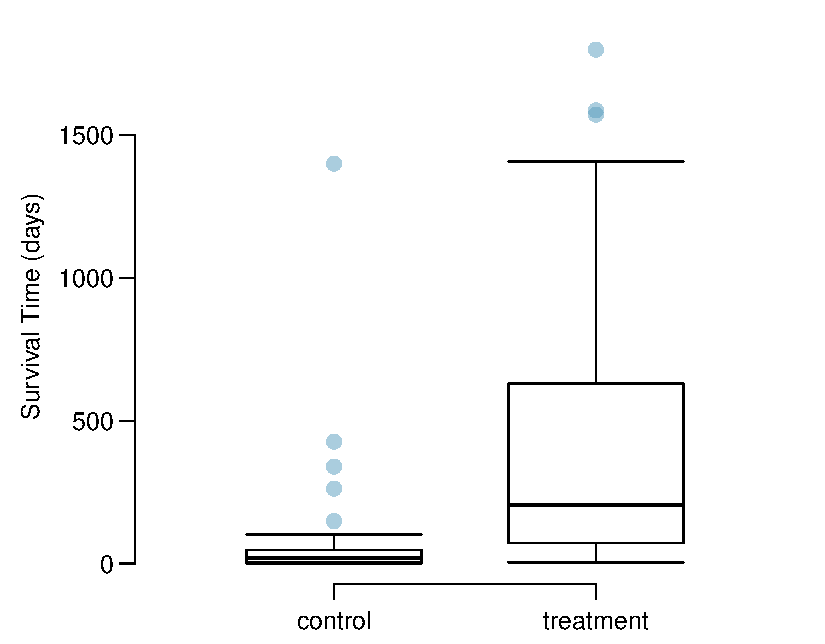
\includegraphics[width = 0.95\textwidth]{01/figures/eoce/heartTr/heartTr_SurvTimeTrBox} \\
\end{center}
\end{minipage}
}
{
\begin{parts}
\item Proportion of patients who are alive at the end of the study is higher in the treatment group than in the control group. These data suggest that survival is not independent of whether or not the patient got a transplant.
\item The shape of the distribution of survival times in both groups is right skewed with one very clear outlier for the control group and other possible outliers in both groups on the high end. The median survival time for the control group is much lower than the median survival time for the treatment group; patients who got a transplant typically lived longer. Tying this together with the much lower variability in the control group, evident by a much smaller IQR than the treatment group (about 50 days versus 500 days), and we can see that patients who did not get a heart transplant tended to consistently die quite early relative to those who did have a transplant. Overall, very few patients without transplants made it beyond a year while nearly half of the transplant patients survived at least one year. It should also be noted that while the first and third quartiles of the treatment group is higher than those for the control group, the IQR for the treatment group is much bigger, indicating that there is more variability in survival times in the treatment group. 
\end{parts}
}\label{HeartTr}

%%%%%%%%%%%%%%%%%%%%%%%%%%%%%%%%%%%%%

\subsection{Case study: efficacy of sulphinpyrazone}

%%%%%%%%%%%%%%%%%%%%%%%%%%%%%%%%%%%%%

% 51

\eoce{\qt{Side effects of Avandia} Rosiglitazone is the active ingredient in the controversial type 2 diabetes medicine Avandia. Rosiglitazone has been linked to an increased risk of serious cardiovascular problems such as stroke, heart failure, and death. A common alternative treatment is pioglitazone, the active ingredient in a diabetes medicine called Actos. In a nationwide retrospective observational study of a cohort of 227,571 Medicare beneficiaries aged  65 years or older, it was found that 2,593 of the 67,593 patients using rosiglitazone and 5,386 of the 159,978 using pioglitazone had serious cardiovascular problems. These data are summarized in the contingency table below. \footfullcite{Graham:2010}
\begin{center}
\begin{tabular}{ll  cc c} 
								&				& \multicolumn{2}{c}{\textit{Cardiovascular problems}} \\
\cline{3-4}	
								&				& Yes 	& No 		& Total	\\
\cline{2-5}
\multirow{2}{*}{\textit{Treatment}}		& Rosiglitazone 	& 2,593	& 65,000		& 67,593 	\\
								& Pioglitazone		& 5,386 	& 154,592 	& 159,978\\
\cline{2-5}
								&Total			& 7,979	& 219,592		& 227,571
\end{tabular}
\end{center}
Determine if each of the below statements is true or false. If false, explain why. \textit{Watch out:} The reasoning may be wrong even if the statement's conclusion is correct. In such cases, the statement should be considered false.
\begin{parts}
\item Since more patients on pioglitazone had cardiovascular problems (5,386 vs. 2,593) we can conclude that rate of cardiovascular problems for those on a pioglitazone treatment is higher.
\item The data suggest that diabetic patients who are taking rosiglitazone are more likely to have cardiovascular problems since the rate of incidence was (2,593 / 67,593 = 0.038) 3.8\% for patients on this treatment, while it was only (5,386 / 159,978 = 0.034) 3.4\% for patients on pioglitazone.
\item The fact that the rate of incidence is higher for the rosiglitazone group proves that rosiglitazone causes serious cardiovascular problems.
\item Based on the information provided so far, we cannot tell if the difference between the rates of incidences is due to a relationship between the two variables or due to chance.
\end{parts}
}
{
\begin{parts}
\item False. Instead of comparing counts, we should compare percentages of people in each group who suffered cardiovascular problems.
\item True.
\item False. Association does not imply causation. We cannot infer a causal relationship based on an observational study. (We cannot say changing the drug a person is on affects her risk, which is why part (b) is true. The difference in these statements is subtle.)
\item True.
\end{parts}
}\label{AvandiaTrueFalse}

% 52

\eoce{\qt{Heart transplants, revisited} Exercise~\ref{HeartTr} introduces the Stanford Heart Transplant Study. Of the 34 patients in the control group, 4 were alive at the end of the study. Of the 69 patients in the treatment group, 24 were alive. The contingency table below summarizes these results.
\begin{center}
\begin{tabular}{ll  cc c} 
							&		& \multicolumn{2}{c}{\textit{Group}} \\
\cline{3-4}
							&		& Control 	& Treatment 	& Total	\\
\cline{2-5}
							& Alive 	& 4	 	& 24			& 28 	\\
\raisebox{1.5ex}[0pt]{\emph{Outcome}} & Dead	& 30		& 45	 		& 75\\
\cline{2-5}
							& Total	& 34		& 69			& 103
\end{tabular}
\end{center}
\begin{parts}
\item What proportion of patients in the treatment group and what proportion of patients in the control group died?
\item One approach for investigating whether or not the treatment is effective is using a randomization technique.
\begin{subparts}
\item What are the claims being tested?
\item  The paragraph below describes the set up for such approach (if we were to do it without using statistical software, which isn't very realistic). Fill in the blanks with a number or word, whichever is appropriate.
\begin{adjustwidth}{2em}{2em}
We write \textit{alive} on \rule{2cm}{0.5pt} cards representing patients who were alive at the end of the study, and \textit{dead} on \rule{2cm}{0.5pt} cards representing patients who were not. Then, we shuffle these cards and split them into two groups: one group of size \rule{2cm}{0.5pt} representing treatment, and another group of size \rule{2cm}{0.5pt} representing control. We calculate the difference between the proportion of \textit{dead} cards in the treatment and control groups (treatment - control) and recod this value. We repeat this many times to build a \rule{2cm}{0.5pt} distribution centered at \rule{2cm}{0.5pt}. Lastly, we calculate the proportion of simulations where the simulated differences in proportions are \rule{2cm}{0.5pt}. If this proportion is low, we conclude that it is unlikely to have observed such an outcome by chance and that the null hypothesis (independence model) should be rejected in favor of the alternative.
\end{adjustwidth}
\item What do the simulation results suggest about the effectiveness of the transplant program?
\end{subparts}
\end{parts}
\begin{center}
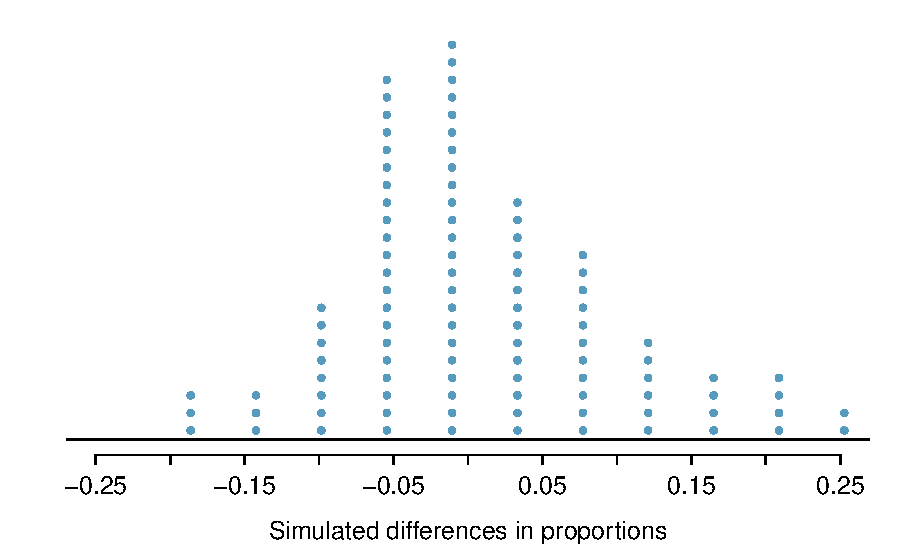
\includegraphics[width = 0.75\textwidth]{01/figures/eoce/heartTr/heartTr_RandHist} \\
\end{center}
}
{
\begin{parts}
\item Proportion of patients who in the treatment group that died: $\frac{45}{69} = 0.652$ \\
Proportion of patients who in the treatment group that died: $\frac{30}{34} = 0.882$
\item 
\begin{enumerate}[i.]
\item $H_0$: Independence model. The variables group and outcome are independent. They have no relationship, and the difference in survival rates between the control and treatment groups was due to chance. In other words, heart transplant is not effective. \\
$H_A$: Alternate model. The variables group and outcome are not independent. The difference in survival rates between the control and treatment groups was not due to chance and the heart transplant is effective.
\item 28, 75, 69, 34, randomization, 0, 0.23 or higher.
\item Under the independence model, only 2 out of 100 times (2\%) did we get a difference of 0.23 or higher between the proportions of patients that died in the treatment and control groups. Since this is a low probability, we can reject the claim of independence in favor of the alternate model. There is convincing evidence to suggest that the transplant program is effective.
\end{enumerate}
\end{parts}
}

% 53

\eoce{\qt{Side effects of Avandia, revisited} Exercise~\ref{AvandiaTrueFalse} introduces a study that compares the rates of serious cardiovascular problems for diabetic patients on rosiglitazone and pioglitazone treatments. The table below summarizes the results of the study.
\begin{center}
\begin{tabular}{ll  cc c} 
								&				& \multicolumn{2}{c}{\textit{Cardiovascular problems}} \\
\cline{3-4}	
								&				& Yes 	& No 		& Total	\\
\cline{2-5}
\multirow{2}{*}{\textit{Treatment}}		& Rosiglitazone 	& 2,593	& 65,000		& 67,593 	\\
								& Pioglitazone		& 5,386 	& 154,592 	& 159,978\\
\cline{2-5}
								&Total			& 7,979	& 219,592		& 227,571
\end{tabular}
\end{center}
\begin{parts}
\item What proportion of all patients had cardiovascular problems?
\item If the type of treatment and having cardiovascular problems were, about how many patients with cardiovascular problems would we have expected in the rosiglitazone group?
\item We can investigate the relationship between outcome and treatment in this study using a randomization technique.  While in reality we would carry out the simulations required for randomization using statistical software, suppose we actually simulate using index cards (as described in Section 1.8.2) \ref{simulatingTheStudy}. In order to simulate from the independence model, which states that the outcomes were independent of the treatment, we write whether or not each patient had a cardiovascular problem on cards, shuffled all the cards together, then dealt them into two groups of size 67,593 and 159,978. We repeat this simulation 1,000 times and each time record the number of people in the rosiglitazone group who had cardiovascular problems. Below is a relative frequency histogram of these counts. \\
\begin{minipage}[c]{0.4\textwidth}
\begin{subparts}
\item What are the claims being tested?
\item Would more or fewer patients with cardiovascular problems in the rosiglitazone group than the number calculated in part (b) provide support for the alternative hypothesis?
\item What do the simulation results suggest about the relationship between taking rosiglitazone and having cardiovascular problems in diabetic patients?
\end{subparts}
\end{minipage}
\begin{minipage}[c]{0.55\textwidth}
\begin{center}
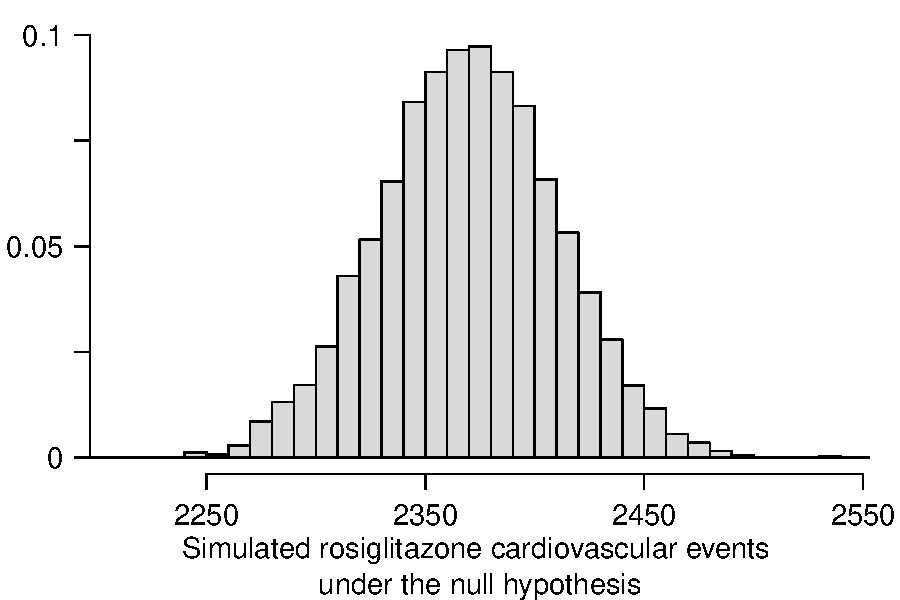
\includegraphics[width = \textwidth]{01/figures/eoce/avandia/avandia_RandHist} \\
\end{center}
\end{minipage}
\end{parts}
}
{
\begin{parts}
\item Proportion of all patients who had a heart attack: $\frac{7,979}{227,571} \approx 0.035$
\item Expected number of heart attacks in the rosiglitazone group if having cardiovascular problems and treatment were independent can be calculated as the number of patients in that group multiplied by the overall cardiovascular problem rate in the study: $67,593 * \frac{7,979}{227,571} \approx 2370$.
\item 
\begin{subparts}
\item $H_0$: Independence model. The treatment and cardiovascular problems are independent. They have no relationship, and the difference in incidence rates between the rosiglitazone and pioglitazone groups is due to chance.
$H_A$: Alternate model. The treatment and cardiovascular problems are not independent. The difference in the incidence rates between the rosiglitazone and pioglitazone groups is not due to chance and rosiglitazone is associated with an increased risk of serious cardiovascular problems.
\item A higher number of patients with cardiovascular problems than expected under the assumption of independence would provide support for the alternative hypothesis as this would suggest that rosiglitazone increases the risk of such problems.
\item In the actual study, we observed 2,593 cardiovascular events in the rosiglitazone group. In the 1,000 simulations under the independence model, we observed somewhat less than 2,593 in every single simulation, which suggests that the actual results did not come from the independence model. That is, the variables do not appear to be independent, and we reject the independence model in favor of the alternative. The study's results provide convincing evidence that rosiglitazone is associated with an increased risk of cardiovascular problems.
\end{subparts}
\end{parts}
}

% 54

\eoce{\qt{Treating sinusitis with a placebo} Researchers studying the effect of antibiotic treatment of acute sinusitis over symptomatic treatments (such as acetaminophen, nasal decongestants, etc) randomly assigned 166 adults diagnosed with sinusitis to two groups. Participants in the antibiotic group received a 10-day course of an antibiotic, and the rest received symptomatic treatments as a placebo. These pills had the same taste and packaging as the antibiotic. At the end of the 10-day period patients were asked if they experienced improvement in symptoms since the beginning of the study. The distribution of responses are summarized below. \footfullcite{Garbutt:2012}
\begin{center}
\begin{tabular}{ll  cc c} 
			&				& \multicolumn{2}{c}{\textit{Self reported}} \\
			&				& \multicolumn{2}{c}{\textit{improvement in symptoms}} \\
\cline{3-4}
			&							& Yes 	& No 	& Total	\\
\cline{2-5}
							&Antibiotic 	& 66	 	& 19		& 85 	\\
\raisebox{1.5ex}[0pt]{\textit{Treatment}}	& Placebo		& 65	 	& 16 	 	& 81 \\
\cline{2-5}
							&Total		& 131	& 35		& 166
\end{tabular}
\end{center}
\begin{parts}
\item What type of a study is this?
\item Does this study make use of blinding?
\item At first glance, does antibiotic or placebo appear to be more effective for the treatment of sinusitis? Explain your reasoning using appropriate statistics.
\item There are two competing claims that this study is used to compare: the independence model and the alternative model. Write out these competing claims in easy-to-understand language and in the context of the application. \textit{Hint:} The researchers are studying the effectiveness of antibiotic treatment.
\item Based on your finding in (c), does the evidence favor the alternative model? If so, what would you do to check if whether this is strong evidence. If not, then explain why.
\end{parts}
}
{
\begin{parts}
\item This is an experiment since patients are randomly assigned to treatment groups.
\item Yes, symptomatic treatments are made to look like antibiotics so that the patients can't tell what treatment they are actually receiving.
\item In the antibiotic group (66 / 85 = 0.776) 77.6\% of patients reported improvement while in the symptomatic treatment group 80.2\% (65/81 = 0.802) did. Improvement rate is 2.6\% higher in the placebo group; therefore at a first glance the placebo appears to be less effective for the treatment of sinusitis.
\item $H_0$: Independence model. The variables treatment and improvement are independent. They have no relationship and the difference in improvement rates between the antibiotic and symptomatic treatment groups is simply due to chance. \\
$H_A$: Alternative model. The variables treatment and improvement are not independent. The difference in improvement rates between the antibiotic and symptomatic treatment groups is not due to chance, and antibiotic is associated with a higher rate of improvement in sinusitis symptoms.
\item No, the evidence does not factor the alternative hypothesis since the proportion of improvement is lower in the antibiotic treatment group.
\end{parts}
}